\documentclass{nuevotema}

\tema{3A-41}
\titulo{Teoría de los ciclos económicos: ciclos nominales y reales.}

\begin{document}

\ideaclave

\seccion{Preguntas clave}

\begin{itemize}
	\item ¿Qué son los ciclos económicos?
	\item ¿Cuáles son las causas de los ciclos económicos?
	\item ¿Qué modelos y métodos existen para explicarlos?
	\item ¿En qué consiste el modelo del ciclo real?
	\item ¿Cómo influyen las variables nominales en las fluctuaciones?
\end{itemize}

\esquemacorto

\begin{esquema}[enumerate]
	\1[] \marcar{Introducción}
		\2 Contextualización
			\3 Macroeconomía
			\3 Fluctuaciones de corto plazo
			\3 Modelos del ciclo económico
		\2 Objeto
			\3 ¿Qué son los ciclos económicos?
			\3 ¿Qué factores causan los ciclos económicos?
			\3 ¿Qué modelos tratan de explicarlos?
			\3 ¿En qué consiste el modelo del ciclo real?
			\3 ¿En qué consisten los modelos del ciclo nominal?
		\2 Estructura
			\3 Hechos estilizados
			\3 Modelos precursores
			\3 Modelo del ciclo real
			\3 Modelo de ciclo monetario: rigideces nominales
	\1 \marcar{Hechos estilizados}
		\2 Idea clave
			\3 Fluctuaciones del PIB
			\3 Afecta a variables de forma simultánea
			\3 Términos frecuentemente utilizados
		\2 Irregularidad
			\3 Ausencia de regularidad
			\3 Grandes variaciones en tamaño de fluctuación
		\2 Componentes de la demanda
			\3 Poco sensibles
			\3 Sensibles
			\3 Contracíclicos
		\2 Asimetría de las fluctuaciones del PIB
			\3 Simetría alrededor de la media
			\3 Duración desigual
		\2 Fases históricas de volatilidad del output
			\3 Patrón Oro (hasta IGM)
			\3 Entreguerras (hasta IIGM)
			\3 Bretton Woods
			\3 Post-Bretton Woods hasta actualidad
			\3 Difícil de distinguir factores
		\2 Correlación de variables con PIB
			\3 Correladas positivamente
			\3 Correladas negativamente
			\3 Ambiguas
		\2 Fechado del ciclo
			\3 Criterios
			\3 Variables utilizadas
	\1 \marcar{Modelos precursores}
		\2 Clásicos
			\3 Idea clave
			\3 Formulación
			\3 Implicaciones
		\2 Marx
			\3 Idea clave
			\3 Implicaciones
		\2 Tugan-Baranovsky
			\3 Idea clave
			\3 Formulación
			\3 Implicaciones
		\2 Austriacos
			\3 Idea clave
			\3 Implicaciones
			\3 Valoración
		\2 Multiplicador-acelerador
			\3 Idea clave
			\3 Formulación
			\3 Implicaciones
		\2 Monetarismo
			\3 Idea clave
			\3 Implicaciones
		\2 Ciclo monetario: información imperfecta
			\3 Idea clave
			\3 Formulación
			\3 Implicaciones
			\3 Valoración
	\1 \marcar{Modelo del ciclo real}
		\2 Idea clave
			\3 Contexto
			\3 Objetivos
			\3 Resultados
		\2 Formulación
			\3 Empresas
			\3 Consumidores
			\3 Gobierno
			\3 Resolución
			\3 Dinámica del equilibrio
			\3 Estimación de shocks tecnológicos
		\2 Implicaciones
			\3 Shocks tecnológico transitorio
			\3 Shocks tecnológico permanente
			\3 Comparación transitorio-permanente en tecnológicos
			\3 Shock transitorio de gasto público
			\3 Shock permanente del gasto público
			\3 Comparación transitorio-permanente en gasto público
			\3 Comparación efectos sobre trabajo
		\2 Extensiones
			\3 Estimación de shocks
			\3 Mercado de trabajo
			\3 Impuestos distorsionantes
			\3 Sectores múltiples
			\3 Dinero
			\3 Ciclos reales endógenos
		\2 Valoración
			\3 Relación con otros modelos
			\3 Cómo valorar capacidad de replicación
			\3 Resultados habituales
			\3 Capacidad de predicción
			\3 Simplificación general ampliable
	\1 \marcar{Ciclo monetario: rigideces nominales}
		\2 Idea clave
			\3 Impulso
			\3 Persistencia
			\3 Eficiencia
			\3 Autores
			\3 Relación con otros modelos
			\3 Estimación de shocks
		\2 Formulación de modelo básico
			\3 Modelo simplificado
			\3 Consumidores
			\3 Empresas
			\3 Equilibrio
			\3 Ecuaciones características
		\2 Implicaciones
			\3 Fluctuaciones en torno a output gap
			\3 Regla de Taylor
			\3 Oferta monetaria exógena
		\2 Valoración
			\3 Capacidad replicativa y explicativa
			\3 Análisis de política monetaria
			\3 Aplicaciones
			\3 Extensiones
	\1[] \marcar{Conclusión}
		\2 Recapitulación
			\3 Hechos estilizados
			\3 Modelos precursores
			\3 Modelo del ciclo real
			\3 Modelo de ciclo monetario: rigideces nominales
		\2 Idea final
			\3 Interés público respecto al ciclo económico
			\3 Los ciclos siempre están presentes
			\3 Otras vías de investigación

\end{esquema}

\esquemalargo














\begin{esquemal}
	\1[] \marcar{Introducción}
		\2 Contextualización
			\3 Macroeconomía
				\4 Análisis de fenómenos económicos a gran escala
				\4 Énfasis sobre variables agregadas
			\3 Fluctuaciones de corto plazo
				\4 Keynes: ``en el largo plazo todos muertos''
				\4[] Pretendía atacar énfasis neoclásico en l/p
				\4[] $\to$ El corto plazo es lo que importa a los agentes
				\4 A c/p, la economía sufre importantes fluctuaciones
				\4 España:
				\4[] PIB real +3,7\% en 2007
				\4[] PIB real -3.9\% en 2009
				\4 Numerosas variables correladas
				\4[] $\to$ Similar patrón de fluctuación
				\4[] Consumo privado
				\4[] Inversión
				\4[] Desempleo
				\4[] ...
				\4[$\Rightarrow$] Las economías no crecen a tasas constantes
				\4[$\Rightarrow$] Fluctúan en torno a tendencias de l/p
				\4[$\Rightarrow$] Estas fluctuaciones son ciclos económicos
			\3 Modelos del ciclo económico
				\4 Representaciones temporales abstractas de macroeconomías
				\4 Muestran fluctuaciones en torno a tendencias
				\4 Se distinguen unos de otros por:
				\4[] $\to$ Factor que impulsa la fluctuación
				\4[] $\to$ Factor que induce persistencia de la fluctuación
		\2 Objeto
			\3 ¿Qué son los ciclos económicos?
			\3 ¿Qué factores causan los ciclos económicos?
			\3 ¿Qué modelos tratan de explicarlos?
			\3 ¿En qué consiste el modelo del ciclo real?
			\3 ¿En qué consisten los modelos del ciclo nominal?
		\2 Estructura
			\3 Hechos estilizados
			\3 Modelos precursores
			\3 Modelo del ciclo real
			\3 Modelo de ciclo monetario: rigideces nominales
	\1 \marcar{Hechos estilizados}
		\2 Idea clave
			\3 Fluctuaciones del PIB
				\4 Alejan PIB de una tendencia central
				\4 Durante varios periodos
				\4 Diferentes a fluctuaciones estacionales
			\3 Afecta a variables de forma simultánea
				\4 Empleo
				\4 Paro
				\4 Productividad
				\4 Inflación
				\4 Salario real
				\4 Tipo de interés
				\4 Oferta monetaria
				\4 ...
			\3 Términos frecuentemente utilizados
				\4 Definen conceptos centrales
				\4[] De modelos modernos del ciclo económico
				\4 Impulso
				\4[] Perturbación que inicia un ciclo
				\4[] Actúa de forma exógena sobre una variable
				\4 Respuesta
				\4[] Variaciones endógenas de las variables del modelo
				\4[] Tras un impulso
				\4 Propagación
				\4[] Fenómeno por el que efectos del impulso
				\4[] Se trasladan de unas variables a otras
				\4 Persistencia
				\4[] Propagación a través del tiempo
				\4[] de efectos del shock
				\4 Amplificación
				\4[] Fenómeno por el que shocks implican respuestas
				\4[] Mayores que el propio shock inicial
				\4 Comovimiento
				\4[] Denota variación en el mismo sentido
				\4[] De dos o más variables afectadas
		\2 Irregularidad
			\3 Ausencia de regularidad
				\4 Una vez las series han sido desestacionalizadas
				\4[] Las fluctuaciones no son cíclicas
				\4[] $\to$ A pesar de nombre ``ciclos económicos''
				\4 Fases de crecimiento y recesión
				\4[] Duración variable
				\4[] Aparentemente aleatoria
			\3 Grandes variaciones en tamaño de fluctuación
				\4[] Tasas de crecimiento/recesión
				\4 En espacio entre fluctuaciones
				\4[] Recesiones muy cortas, largas, etc...
		\2 Componentes de la demanda
			\3 Poco sensibles
				\4 Consumo de bienes perecederos
				\4 Consumo de servicios
				\4 A pesar de que representan mayor \% de PIB
				\4[] $\to$ fluctúan menos que resto de componentes
			\3 Sensibles
				\4 Inventarios/Existencias
				\4[] Muy poco \% sobre PIB
				\4[] Pero fluctuaciones elevadas en propio \%
				\4[] Fuertes aumentos en inicio recesión
				\4[] Fuertes caídas en salida recesión
				\4 FBKF no residencial
				\4[] Fuerte caída en recesión
				\4 FBKF en vivienda
				\4[] Caídas en recesiones
			\3 Contracíclicos
				\4 Posiblemente gasto público
				\4[] No siempre
				\4[] Otros factores determinan
				\4[] $\to$ Posición fiscal
				\4[] $\to$ Sector exterior
				\4 Exportaciones netas en algunos casos
				\4[] Especialmente cuando recesión tiene origen interno
				\4[$\to$] Crecen o se mantienen durante recesiones
		\2 Asimetría de las fluctuaciones del PIB
			\3 Simetría alrededor de la media
				\4 Valles y picos
				\4[] Aproximadamente misma cuantía
			\3 Duración desigual
				\4 Recesiones en general más cortas
				\4 Recuperaciones más largas
				\4[] $\Rightarrow$ Crecimiento de largo plazo
		\2 Fases históricas de volatilidad del output\footnote{Basado en Basu y Taylor (1999).}
			\3 Patrón Oro (hasta IGM)
				\4[] $\to$ Volatilidad media
			\3 Entreguerras (hasta IIGM)
				\4[] $\to$ Volatilidad elevada
			\3 Bretton Woods
				\4[] $\to$ Volatilidad media
			\3 Post-Bretton Woods hasta actualidad
				\4 Generalmente
				\4[] $\to$ Volatilidad reducida
				\4 Gran Recesión
				\4[] Contracción muy fuerte
			\3 Difícil de distinguir factores
				\4 Cambios no son dramáticos
				\4 Series de datos limitadas
				\4 ¿Cambio sectorial?
				\4 ¿Factores que se compensan unos a otros?
		\2 Correlación de variables con PIB
			\3 Correladas positivamente
				\4[] Empleo
				\4[] Horas trabajadas
				\4[] Tipo de interés nominal
				\4[] Tipo de interés real
			\3 Correladas negativamente
				\4[] Paro
			\3 Ambiguas
				\4 Productividad
				\4[] Determinadas economías aumentan productividad
				\4[] $\to$ Más despidos que caída del PIB
				\4[] En general, productividad baja en recesiones
				\4 Inflación
				\4[] En media, generalmente bajadas débiles
				\4 Salarios
				\4[] Débilmente procíclicos
		\2 Fechado del ciclo
			\3 Criterios
				\4 Variables
				\4 A menudo, comités nacionales emiten opiniones
				\4 Asoc. Española de Economía -- ``Comité de Fechado''
				\4 Business Cycle Dating Committee -- NBER
			\3 Variables utilizadas
				\4 PIB ocupa lugar principal
				\4[] Pero no único
				\4 Consumo privado, FBKF, empleo, etc...
				\4 No hay reglas fijas para definir recesión
				\4[] En ocasiones, criterio de los dos trimestres
				\4[] $\to$ Dos trimestres de crecimiento negativo
	\1 \marcar{Modelos precursores}
		\2 Clásicos
			\3 Idea clave
				\4 Sin modelo explícito canónico
				\4 Tendencia a estabilidad
				\4
			\3 Formulación
				\4 Ley de Say
				\4[] No pueden existir excesos agregados de demanda
				\4[] $\to$ Se corrigen sólos
				\4 Cambios tecnológicos
				\4[] Reajuste de oferta y demanda
				\4[] $\to$ Equilibrio
				\4 Cambios en distribución de renta
				\4[] Reajuste de oferta y demanda
				\4[] $\to$ Equilibrio
			\3 Implicaciones
				\4 Estabilización del ciclo indeseable
				\4[] Más problemas de los solucionados
				\4 Ciclos eminentemente exógenos
		\2 Marx
			\3 Idea clave
				\4 Ciclos endógenos
				\4 $\uparrow$ salarios como inicio del ciclo
				\4[] Se reduce plusvalía
				\4[] Cae inversión $\to$ Cae demanda agregada
				\4[] Precios caen
				\4[] Tasa de beneficio cae más
				\4[] Inversión vuelve a caer
				\4[] $\to$ Cae demanda agregada
				\4[] Crisis se agudiza
				\4[] Empresas ineficientes desaparecen
				\4[] $\uparrow$ desempleo
				\4[] $\uparrow$ Ejército industrial de reserva
				\4[] $\uparrow$ Productividad
				\4[] $\uparrow$ Tasa de beneficio
				\4[] $\uparrow$ Inversión $\to$ $\uparrow$ demanda agregada
				\4[] $\uparrow$ Salarios
				\4[] ...
			\3 Implicaciones
				\4 Ciclo es proceso endógeno
				\4 Economía capitalista inestable
				\4 Crisis cada vez peores
				\4 Tendencia autodestructiva del sistema
		\2 Tugan-Baranovsky
			\3 Idea clave
				\4 Ley de Say predominante en s. XIX
				\4[] Fluctuaciones cíclicas son shocks externos
				\4 No siempre se observan shocks
				\4[] $\to$ ¿Cómo explicar?
				\4[] $\then$ ¿No hay shocks?
				\4[] $\then$ ¿No son shocks la causa?
				\4[] $\then$ ¿No somos capaces de observarlos?
				\4 Tugan-Baranovsky:
				\4[] $\to$ Mecanismo que da lugar a fluctuación
				\4[] $\then$ Sin shock externo
			\3 Formulación
				\4 Economía crece
				\4[] Beneficios aumentan
				\4 Capitalistas invierten beneficios en K físico
				\4[] Aumenta demanda agregada y empleo
				\4[] $\to$ Agotan fondos prestables disponibles
				\4[] $\then$ Suben tipos de interés
				\4[] Subida de tipos de interés
				\4[] $\to$ Reduce demanda de inversión
				\4[] $\then$ Exceso de oferta de bienes de capital
				\4 Caen ventas por exceso de oferta agregado
				\4[] Caen ingresos
				\4[] $\to$ Caen inversión en capital y préstamo
				\4 Ahorro se mantiene constante
				\4[] Menos demanda de inversión que ahorro
				\4[] $\to$ Tipos de interés caen
				\4[] $\then$ Proceso empieza de nuevo
			\3 Implicaciones
				\4 Ciclos son inherentes a capitalismo
				\4[] Crítica a Ley de Say
				\4[] $\to$ Ciclos no resultan de shocks externos
				\4 Capitalismo se corrige a sí mismo
				\4[] Al contrario que Marx
				\4[] $\to$ Economía capitalista no sigue proceso degenerativo
		\2 Austriacos
			\3 Idea clave
				\4 Hayek (Nobel en 1974), Von Mises
				\4[] Influenciados por Wicksell
				\4[] $\to$ Proceso acumulativo de Wicksell
				\4[] $\then$ Interés monetario por debajo de natural
				\4[] $\then$ Exceso de inversión
				\4[] $\then$ Inflación
				\4 Exceso de crédito es causa de ciclos
				\4 Política monetaria demasiado laxa
				\4[] Bancos centrales compran mucho papel
				\4[] Oferta monetaria aumenta
				\4[] Interés efectivo por debajo de natural
				\4[] $\to$ Influencia Wickselliana
				\4 Inversión excesiva
				\4[] Por interés nominal inferior a natural
				\4[] Proyectos poco rentables se llevan a cabo
				\4[] Mala asignación de recursos
				\4 Inversores ajustan carteras
				\4[] Venden proyectos poco rentables
				\4[] Reacción en cadena
				\4[] Cae precio de activos
				\4[] Suben tipos de interés
				\4[] Demanda agregada se desploma
				\4[$\then$] Recesión
				\4 Ciclo comienza de nuevo
			\3 Implicaciones
				\4 Ajuste más costoso cuanto más tardío
				\4[] Más inversiones ineficientes
				\4[] Más ajuste de precios
				\4 Política monetaria causa crisis
				\4[] Defienden free-banking
				\4[] Contra reserva fraccionaria
			\3 Valoración
				\4 Numerosas críticas
				\4 No falsable
				\4[] Problema similar a ciclo marxista
				\4[] No excluye ningún estado de la naturaleza
				\4 Empíricamente, inversión neta positiva
				\4[] Casi siempre
				\4[] A pesar de crisis
				\4[] Pero según modelo, debería haber desinversión
				\4 Cuantificación de interés natural
				\4[] Imposible
				\4[] $\to$ ¿Cómo valorar optimalidad de política monetaria?
		\2 Multiplicador-acelerador\footnote{Ver \href{https://python.quantecon.org/samuelson.html}{Sargent y Stachurski: Application: The Samuelson Multiplier-Accelerator} y \href{https://muse.jhu.edu/article/13350/pdf}{Heertje y Heemeijer (2002) On the Origin of Samuelson's Multiplier-Accelerator Model}.}
			\3 Idea clave
				\4 Contexto
				\4[] Concepto clásico del ciclo
				\4[] $\to$ Shocks endógenos
				\4[] Modelos marxista y austríaco
				\4[] $\to$ Escasa formalización
				\4[] $\to$ Problemas de falsabilidad
				\4[] $\to$ Impulso endógeno
				\4[] Keynes
				\4[] $\to$ Excesos agregados de demanda posibles
				\4[] $\to$ Formalización incipiente
				\4[] $\to$ Demanda agregada relevante
				\4[] Hansen, Hicks
				\4[] $\to$ Formulación de SS-LL
				\4[] $\to$ Precedesores de IS-LM
				\4[] Harrod
				\4[] $\to$ Keynesianismo aplicado al crecimiento
				\4[] Harrod (1936) y Samuelson (1939)
				\4 Objetivos
				\4[] Modelo formal de ciclo endógeno
				\4[] Cuantificación de parámetros determinantes
				\4[] Valorar efecto de impulsos exógenos sobre ciclo endógeno
				\4 Resultados
				\4[] Primer modelo formal de ciclo endógeno
				\4[] Dinamización de modelo keynesiano
				\4[] Fuerte impacto en política económica
				\4[] Inspiración de modelos macroeconométricos de ciclo
				\4[] Elementos característicos
				\4[] i. Multiplicador del consumo
				\4[] $\to$ Consumo depende de ingreso pasado
				\4[] $\then$ Más ingreso pasado, aumenta consumo presente
				\4[] ii. Acelerador
				\4[] $\to$ Inversión depende de ingreso
				\4[] $\to$ Relación fija de capital inversión
				\4[] Parámetros determinan dinámica
				\4[] $\to$ Propensión al consumo
				\4[] $\to$ Relación capital ahorroº
				\4[] Shocks exógenos pueden impulsar
				\4[] $\to$ Animal spirits que afectan consumo
				\4[] $\to$ Gasto público
			\3 Formulación
				\4 Output total
				\4[] $Y_t = C_t + I_t + G_t$
				\4 Consumo: multiplicador
				\4[] $C_t = \alpha Y_{t-1} + \gamma$
				\4 Inversión: acelerador
				\4[] $I_t = \beta \left( Y_{t-1} - Y_{t-2} \right)$
				\4 Gasto público
				\4[] $G_t = G_0$
				\4[$\then$] $Y_t = (\alpha +\beta) Y_{t-1} - \beta Y_{t-2} + \gamma + G_t$
				\4 Decisión de inversión de las empresas
				\4[] Respecto a output pasados
				\4[] $\to$ Como estimación de output que se necesitará
				\4[] $\then$ Lags de la inversión
				\4 Multiplicador del gasto
				\4[] Demanda de gasto genera aumento de output
				\4[] Demanda de gasto depende output
				\4[] $\to$ Más gasto induce más output
				\4[] $\then$ Más gasto retroalimenta aumento de demadna
				\4[] Demanda tiene efecto multiplicador sobre output
				\4[] $\to$ Superior a 1
				\4[] $\then$ 1 ud. más de gasto, aumenta output > 1
				\4 Ajuste dinámico
				\4[] Consumo e inversión dependen de $Y_{t-1}$
				\4[$\then$] Interacción dinámica entre variables
				\4 Generación de ciclos
				\4[] Caída de demanda en un momento dado
				\4[] $\to$ Animal spirits
				\4[] $\to$ Otros factores
				\4[] Inversión depende de periodos pasados
				\4[] $\to$ Lags de inversión
				\4[] Exceso de inversión
				\4[] $\to$ Caída posterior de inversión
				\4[$\then$] Aparición de ciclos
			\3 Implicaciones
				\4 Shocks exógenos modelizables
				\4[] Animal spirits vía $\gamma$
				\4[] Gasto público vía $G_t$
				\4 Acelerador de la inversión
				\4[] Asumiendo relación fija K-Y
				\4[] $\uparrow Y$ implica $\uparrow$ proporcional de K
				\4 Ciclos endógenos posibles
				\4[] Amplitud creciente o decreciente
				\4[] Depende de parámetros
				\4 Ciclos endógenos amplitud constante
				\4[] Posible encontrar valor de equilibrio
				\4[] Valor sobre ``razor-edge''
				\4 Fluctuaciones explosivas
				\4[] Con mínimo impulso inicial
		\2 Monetarismo
			\3 Idea clave
				\4 Mejor fluctuaciones que ciclos
				\4[] Critica término ``ciclos''
				\4 Ciclos son fundamentalmente monetarios
				\4 Friedman (1964) Posibilidad de ciclos ``plucking''\footnote{\href{https://www.bruegel.org/2015/02/the-plucking-model-of-recessions-and-recoveries/}{Ver Bruegel sobre modelos ``plucking''.}}
				\4[] No son desviaciones respecto tendencia
				\4[] $\to$ Arriba y abajo respecto tendencia
				\4[] $\then$ Modelo de ciclos basado en output ``natural''
				\4[] $\then$ Plucking como alternativa
				\4[] Ciclos son impulsos que alejan de techo máximo
				\4[] $\to$ Siempre alejado por sucesión de impulsos
				\4[$\then$] Si Plucking correcto:
				\4[] Recesiones más fuertes, expansión más fuerte
				\4[$\then$] Si basada en output natural correcto:
				\4[] Recesiones más cortas, expansiones más cortas
				\4[] $\to$ Tamaño de recesiones predice tamaño expansiones
				\4[] También posible expansión débil pero más larga?
			\3 Implicaciones
				\4 PM basada en oferta monetaria
				\4 Regla de oferta monetaria
				\4[] Predecible y conocida
				\4[] Crecimiento de M fijado por ley
		\2 Ciclo monetario: información imperfecta
			\3 Idea clave
				\4 Primer modelo microfundamentado
				\4[] Consumidores-productores optimizan decisiones
				\4[] Resiste a crítica de Lucas
				\4[] $\to$ Más apto para análisis de políticas
				\4 Marco walrasiano
				\4[] Pionero
				\4[] Mercados siempre en equilibrio
				\4[] Ciclo no es trayectoria hacia equilibrio
			\3 Formulación
				\4 Optimización de los trabajadores
				\4[] Trabajdores deben extraer señales
				\4[] $\to$ Observan precio individual
				\4[] $\to$ No conocen precio agregado
				\4[] $\to$ Conocen estructura de la economía
				\4[] $\then$ ¿Qué precio relativo tiene mi output?
				\4[] $\then$ ¿$\Delta$ PRelativo es permanente o transitoria?
				\4[] A partir de:
				\4[] $\to$ PRelativo estimado
				\4[] $\to$ Expectativa de duración de $\Delta$ PRelativo
				\4[] Deciden:
				\4[] $\to$ Cuánto trabajar hoy y mañana
				\4[] $\to$ Cuánto invertir en capital hoy
				\4 Inversión en capital
				\4[] Invierten parte del salario
				\4[] Aumentan productividad en periodos futuros
				\4 Lags de las expectativas
			\3 Implicaciones
				\4 Inversión en capital no es reversible
				\4[] Shocks tienen efectos persistentes
				\4[] $\to$ Aunque shocks no lo sean
				\4 Desequilibrio no existe
				\4 Desempleo no existe
				\4 Ciclos son óptimos paretianos
				\4 Estabilización no es deseable
			\3 Valoración
				\4 Precursor de modelos RBC
				\4[] Siempre en equilibrio
				\4[] Equilibrios son óptimos
				\4 Precursor de DSGE
				\4[] Dinero provoca fluctuaciones reales
	\1 \marcar{Modelo del ciclo real}\footnote{Basado fundamentalmente en Sims, E. (2015) \textit{Graduate Macro Theory II: Fiscal Policy in the RBC Model.} Sincronizar con 3A-37 sobre política fiscal y 4B-5 sobre presupuesto público como instrumento compensador de la actividad económica.}
		\2 Idea clave
			\3 Contexto
				\4 Modelos de NMC
				\4[] $\to$ Macroeconomía es equilibrio general walrasiano
				\4[] Crítica de Lucas
				\4[] $\to$ Microfundamentación para tratar de evitar
				\4[] Modelo neoclásico de crecimiento
				\4[] $\to$ Referencia básica
				\4 Autores
				\4[] Kydland y Prescott (1982)
				\4[] Long y Plosser (1983)
				\4[] Otros nombres:
				\4[] $\to$  King, Rebelo, Benhabib, ...
			\3 Objetivos
				\4 Formular modelo cuantitativo de efecto de shocks
				\4 Shocks exclusivamente reales
				\4 Replicar momentos de macromagnitudes principales
				\4[] Varianza
				\4[] Correlaciones
				\4[] $\then$ Con modelo robusto a crítica de Lucas
			\3 Resultados
				\4 Modelo de eg. walrasiano
				\4 Dicotomía clásica
				\4[] Curva de Phillips perfectamente vertical
				\4 Impulso
				\4[] Shocks estocásticos sobre variables reales
				\4[] $\to$ Tecnología
				\4[] $\to$ Gasto público
				\4[] Variables nominales no son tenidas en cuenta
				\4[] Dicotomía clásica perfecta
				\4 Persistencia
				\4[] Autocorrelación de shocks
				\4[] $\to$ Persistencia por definición
				\4[] Inversión en capital
				\4[] $\to$ Persistencia indirecta
				\4 Capital
				\4[] Los agentes acumulan capital
				\4[] Acumulación de capital afecta a producción
				\4[] $\to$ Permite autocorrelación del output
				\4[] $\to$ Permite representar efecto acelerador
				\4 Equilibrio
				\4[] Resultado de optimización estocástica con HER
				\4[] Optimización consumo-ocio intratemporal
				\4[] Optimización consumo-ocio intertemporal
				\4 Eficiencia
				\4[] Desviaciones respecto de la tendencia
				\4[] Son también equilibrios dinámicos
				\4[] No son trayectorias de ajuste hacia eq. eficiente
				\4[] $\to$ Los mercados están en equilibrio en todos los periodos
				\4[] $\to$ Ajuste perfectamente flexible de precios
				\4[] $\to$ Trayectorias de equilibrio son óptimos de Pareto
		\2 Formulación
			\3 Empresas
				\4 Maximización de los beneficios de las empresas
				\4[] Decidiendo sobre:
				\4[] $\to$ Capital
				\4[] $\to$ Trabajo
				\4[] $\underset{N_t, K_t}{\max} \quad \Pi_t = \underbrace{A_t K_t^\alpha N_t^{1-\alpha}}_{Y_t} - w_t N_t - R_t K_t$
				\4[] CPO: \quad $w_t = (1-\alpha) A_t K_t^\alpha N_t^\alpha$
				\4[] \quad \quad $R_t = \alpha A_t K_t^{\alpha-1} N_t^{1-\alpha}$
				\4[] Donde:
				\4[] $\to$ $A_t = (1-\rho)A\cdot e^{gt} + \rho_A A_{t-1} + \epsilon_t$
			\3 Consumidores
				\4 Maximización de la utilidad de los consumidores
				\4[] Decidiendo sobre:
				\4[] $\to$ Consumo en periodo
				\4[] $\to$ Trabajo en periodo
				\4[] $\to$ Capital en periodo
				\4[] $\to$ Inversión en activo del gobierno en periodo
				\4[] $\underset{C_t, N_t,K_t, B_t}{\max} \quad \sum_{t=0}^\infty \beta^t u(C_t, N_t)$
				\4[] $\text{s.a}: \quad C_t+\underbrace{K_t - (1-\delta)K_{t-1}}_{I_t} + B_t - (1+r_{t-1})B_{t-1} \leq$
				\4[] \quad \quad \quad $\leq \underbrace{wN_t + R_t K_t + \Pi_t}_{Y_t} - T_t$
				\4[] \quad \quad \quad $\lim_{T \to \infty}  K_t \geq 0$
				\4[] \quad \quad \quad $\then$ $\sum_{t=0}^\infty \frac{C_t + I_t}{(1+r)^t} = \sum_{t=0}^\infty \frac{ Y_t}{(1+r)^{t}} - \sum_{t=0}^\infty \frac{T_t}{(1+r)^{t}}$
				\4[] Donde:
				\4[] $\to$ $u(C_t, N_t) = \left( \ln C_t  - v(N_t) \right)$
				\4[] CPO: \quad $u'(C_t) = \beta u'(C_{t+1})$
				\4[] \quad \quad $w_t = \frac{u_{N_T}}{u_{C_t}}$
			\3 Gobierno
				\4 Senda exógena de gasto público sujeta a restricción
				\4[] $G_t + r_{t-1} D_t \leq T_t + D_{t+1} - D_t$
				\4[] $\to$ $T_t = G_t - \left( D_t - (1+r_{t-1} D_{t-1}) \right)$
				\4[] Condición de No-Ponzi + Transversalidad
				\4[] $\then$ $\sum_{t=0}^\infty \frac{G_t}{(1+r)^t} = \sum_{t=0}^\infty \frac{T_t}{(1+r)^t}$
			\3 Resolución
				\4 Resolución por método de Lagrange
				\4[] Si secuencia de shocks es conocida
				\4[] $\to$ $\epsilon_t$ a productividad
				\4[] $\to$ $G_t$ a gasto público
				\4 Resolución por programación dinámica
				\4[] Si shocks aleatorios
			\3 Dinámica del equilibrio
				\4[] $u'(C_t) = \beta u'(C_{t+1})$
				\4[] $w_t = \frac{u_{N_T}}{u_{C_t}}$
				\4[] $C_t + I_t + G_t = Y_t$
				\4[] $I_t = K_{t+1} - (1-\delta) K_t$
				\4[$\then$] Estado estacionario: secuencias de vars. exógenas
				\4[] $C_t = C(K_t, \left\lbrace A_t \right\rbrace^\infty_0, \left\lbrace G_t \right\rbrace )$
				\4[] $N_t = N(K_t, \left\lbrace A_t \right\rbrace^\infty_0, \left\lbrace G_t \right\rbrace )$
				\4[] $K_t = K (K_t, \left\lbrace A_t \right\rbrace^\infty_0, \left\lbrace G_t \right\rbrace )$
				\4 Aproximación y log-linearización
				\4[] Solución suele tomar forma de
				\4[] sistema de eqs. parciales diferenciales
				\4[] $\to$ Sin solución analítica en forma cerrada
				\4[] $\to$ Aproximación de la solución y linearización
				\4 Ecuaciones de dinámica aproximada
				\4[] Tras linearización del estado estacionario
				\4[] $\tilde{C}_{t+1} = a_{CK}\tilde{K}_{t+1} + a_{CA}\tilde{A}_{t+1} + a_{CG} \tilde{G}_{t+1}$
				\4[] $\tilde{L}_{t+1} = a_{LK}\tilde{K}_{t+1} + a_{LA}\tilde{A}_{t+1} + a_{LG} \tilde{G}_{t+1}$
				\4[] $\tilde{K}_{t+1} = b_{KK}\tilde{K}_{t} + b_{KA}\tilde{A}_{t} + b_{KG} \tilde{G}_{t}$
				\4 Parámetros de las ecuaciones de dinámica
				\4[] Derivados de parámetros estructurales exógenos
				\4[] Entre ellos:
				\4[] $\alpha$: elasticidad-capital del output
				\4[] $g$: tasa de crecimiento tendencial
				\4[] $\rho$: tasa de descuento de la utilidad
				\4[] $\rho_\theta$: persistencia del shock de productividad
				\4[] tipo de interés de equilibrio
				\4[] etc...
			\3 Estimación de shocks tecnológicos
				\4 Shocks tecnológicos
				\4[] Pueden representar perturbaciones sobre:
				\4[] $\to$  Productividad
				\4[] $\to$ Liberalización y desregulación
				\4[] $\to$ Desastres naturales o guerras
				\4 Filtros de tendencias
				\4[] Métodos matemáticos para extraer
				\4[] $\to$ Componente cíclico
				\4[] $\then$ Shocks de productividad
				\4 Estimados mediante diferentes filtros
				\4[] Descomponer tendencia+ciclo
				\4[] Univariables
				\4[] $\to$ A partir de una variable
				\4[] $\to$ Generalmente, PIB
				\4[] Multivariables
				\4 Filtro de Hodrick-Prescott
				\4[] Hallar secuencia de output tendencia
				\4[] $\to$ Que minimiza función de pérdida
				\4[] Función de pérdida penaliza de:
				\4[] $\to$ Diferencia entre output y tendencia
				\4[] $\to$ Variaciones entre periodos de tendencia
				\4[] $\then$ Parametrizable para variar peso de uno y otro
				\4[] Dibujar gráfica $y$--$t$ y tendencia superpuesta
				\4[] $\tilde{C}_t$, $\tilde{K}_{t+1}$, $\tilde{N}_t$
				\4[] $\to$ Expresan diferencias frente a tendencia
		\2 Implicaciones
			\3 Shocks tecnológico transitorio
				\4 Aumenta tipo de interés
				\4[] Aumenta productividad marginal del capital
				\4[] $\uparrow$ Interés reduce a medida que capital aumenta
				\4 Aumenta salario
				\4[] Aumenta productividad marginal del trabajo
				\4[] Aumento se mantiene por aumento de capital
				\4 Trabajan más horas en presente y menos en futuro
				\4[] Asumiendo ES más importante que ER
				\4 Aumentan consumo presente y futuro
				\4[] $\to$ Pero aumento tiende a disiparse
				\4 Aumenta el ahorro presente
				\4[] Para suavizar consumo
				\4[] $\Rightarrow$ Aumenta capital
				\4 Producto crece varios periodos
				\4[$\Rightarrow$] Correlación positiva:
				\4[] Salario real y output\footnote{Aunque si la oferta de trabajo es muy elástica al salario, puede aumentar tanto que el salario real caiga.}
				\4[] Horas trabajadas y productividad
				\4[] Productividad y output
				\4[] Interés y output
				\4[] Inversión y output
				\4 Representación gráfica
				\4[] \grafica{rbcefectodynareptftransitorio}
			\3 Shocks tecnológico permanente
				\4 Aumenta tipo de interés
				\4[] Aumenta productividad marginal del capital
				\4[] $\uparrow$ Interés reduce a medida que K aumenta
				\4[] $\to$ Más inversión porque shock es permanente
				\4 Aumenta salario presente y futuro
				\4[] ER $\sim$ ES $\to$ Efecto ambiguo sobre empleo
				\4 Aumenta consumo de forma permanente
				\4 Aumenta capital de forma permanente
				\4 Producto crece de forma permanente
				\4[] Pero reacciona menos que si transitorio
				\4[] $\to$ Porque menor aumento de empleo
				\4 Efectos similares a $\uparrow$ productividad en RCK
				\4[] Nuevo estado estacionario
				\4[] $f'(k) = \rho + \theta g$
				\4[] $c=f(k) -(n+g)k$
				\4 Representación gráfica
				\4[] \grafica{rbcefectodynareptfpermanente}
			\3 Comparación transitorio-permanente en tecnológicos\footnote{De Sims (2016).}
				\4 Cuanto más persistente sea el shock:
				\4[Consumo] + $\uparrow$ sobre consumo
				\4[Tratajo] -- aumento del trabajo
				\4[Salarios] + $\uparrow$ los salarios
				\4[Output] -- reacción transitoria del output
				\4[Inversión] -- reacciona la inversión
				\4[Tipo de interés] + $\uparrow$ el tipo de interés
			\3 Shock transitorio de gasto público
				\4 Supuestos:
				\4[] gasto público improductivo
				\4[] Impuesto de suma fija no distorsionante
				\4 Output aumenta
				\4[] $\to$ Aunque mucho menos que gasto público
				\4 Consumo cae
				\4[] $\to$ Muy ligeramente
				\4 Inversión cae
				\4[] Caída muy pronunciada y recuperación rápida
				\4 Trabajo aumenta
				\4[] Muy ligeramente
				\4[] $\to$ Sin efecto sustitución ocio-consumo
				\4[] $\to$ Pequeño efecto renta
				\4 Salarios caen
				\4[] Muy ligeramente
				\4[] $\to$ Aumento de oferta de trabajo
				\4[] $\to$ Menos capital
				\4[] $\to$ Igual productividad
				\4 Tipo de interés
				\4[] Aumenta muy ligeramente
				\4 Representación gráfica
				\4[] \grafica{rbcefectodynaregastotransitorio}
			\3 Shock permanente del gasto público
				\4 Supuestos:
				\4[] gasto público improductivo
				\4[] Impuesto de suma fija no distorsionante
				\4 Output aumenta
				\4[] Más que con shock transitorio
				\4 Consumo cae
				\4[] Más que con shock transtorio
				\4 Inversión cae
				\4[] Más que con shock transitorio
				\4[] De manera más persistente
				\4 Trabajo aumenta
				\4[] Más que con shock transitorio
				\4[] $\to$ Efecto renta mucho mayor ahora
				\4[] $\to$ Sin efecto sustitución ocio-consumo
				\4 Salarios caen
				\4[] Más que en transitorio
				\4[] $\to$ Aumento de la oferta de trabajo
				\4[] $\to$ Menos capital
				\4[] $\to$ Igual productividad
				\4 Tipo de interés
				\4 Representación gráfica
				\4[] \grafica{rbcefectodynaregastopermanente}
			\3 Comparación transitorio-permanente en gasto público
				\4 Cuanto más persistente sea el shock:
				\4[Consumo] + $\uparrow$ sobre consumo
				\4[Trabajo] + aumento del trabajo
				\4[Salarios] + $\downarrow$ los salarios
				\4[Output] + aumenta el output
				\4[Inversión] + persistente caída de la inversión
				\4[Tipo de interés] + $\uparrow$ el tipo de interés
			\3 Comparación efectos sobre trabajo
				\4 Shock productividad
				\4[] Transitorio:
				\4[] $\to$ $\left| \text{ES} + \text{ER}_i\right|$: elevado
				\4[] $\to$ $\text{ER}_D$: muy pequeño
				\4[] $\then$ Más probable que $\frac{d \, h}{d \, w} > 0$
				\4[] $\then$ Aumento fuerte de oferta de trabajo
				\4[] Permanente:
				\4[] $\to$ $\left| \text{ES} + \text{ER}_i\right|$: elevado
				\4[] $\to$ $\text{ER}_D$: elevado
				\4[] $\then$ ER directo compensa ES+ER indirecto
				\4[] $\then$ Menor aumento de oferta de trabajo
				\4 Shock gasto público
				\4[] Transitorio:
				\4[] $\to$ $\left| \text{ES} + \text{ER}_i\right|$: sin efecto
				\4[] $\to$ $\text{ER}_D$: muy pequeño
				\4[] $\then$ Más probable que $\frac{d \, h}{d \, w} > 0$
				\4[] $\then$ Aumento fuerte de oferta de trabajo
				\4[] Permanente:
				\4[] $\to$ $\left| \text{ES} + \text{ER}_i\right|$: sin efecto
				\4[] $\to$ $\text{ER}_D$: creciente cuanto más permanente
				\4[] $\then$ ER directo compensa ES+ER indirecto
				\4[] $\then$ Menor aumento de oferta de trabajo
				\4 Tabla resumen
				\4[] \grafica{resumenefectostrabajo}
		\2 Extensiones
			\3 Estimación de shocks
				\4 Residuo de Solow como estimación de shocks de prod.
				\4[] $\to$ Recibe críticas: necesarios shocks muy grandes
				\4[] $\to$ Crisis implican shocks negativos muy grandes
			\3 Mercado de trabajo
				\4 Rogerson (1984), Hansen (1985)
				\4 Trabajo indivisible
				\4[] $\to$ Cambios en trabajo no son sólo cambios en horas
				\4[] $\then$ Sobre todo, cambios en número de empleados
				\4 Incorporar respuesta de trabajo a shocks
				\4[] $\to$ Shocks implica variación más fuerte de trabajo
				\4[] $\Rightarrow$ Baja respuesta de horas trabajadas a shock
				\4[] $\Rightarrow$ Mejoran replicación de series reales
			\3 Impuestos distorsionantes\footnote{Pág. 230 de Romer.}
				\4 Puede introducir efectos de sustitución temporal
				\4 Puede distorsionar
				\4[] rendimientos relativos trabajo y capital
				\4[] $\to$ Equivalencia ricardiana
			\3 Sectores múltiples
				\4[] Efectos de transmisión de shocks entre sectores
				\4[] Estructura de mercados determina respuesta a shocks
			\3 Dinero
				\4[] En RBC, perturbaciones monetarias
				\4[] $\to$ Afectan sólo a variables nominales
				\4[] RBC se abstrae de perturbaciones monetario-real
				\4[] En la práctica
				\4[] $\to$ Perturbaciones monetarias afectan reales
				\4[] Modelos de ciclo nominal o monetario
			\3 Ciclos reales endógenos
				\4[] Benhabib y Nishimura (1985)
				\4[] Conectados con crecimiento endógeno
				\4[] No hay convergencia a un estado estacionario
				\4[] El propio modelo genera fluctuaciones endógenas
		\2 Valoración
			\3 Relación con otros modelos
				\4 Basado en Ramsey (1926), y Cass y Koopmans
				\4 Culmina programa de investigación de Lucas:
				\4[] Formular ciclo económico en marco de equilibrio
				\4[] Ciclos como óptimos de Pareto
				\4[] Sin supuestos no walrasianos ad-hoc
				\4[] $\to$ Mercados deben vaciarse
				\4 Consolidación de marco DSGE
				\4[] iniciado por Lucas 1972
				\4[] optimización Dinámica de los agentes
				\4[] sujetos a impulsos eStocásticos
				\4[] en contexto de Equilibrio General
			\3 Cómo valorar capacidad de replicación
				\4[1] Calibración del modelo
				\4[] Elegir valores de parámetros en base a:
				\4[] $\to$ Teoría microecómica
				\4[] $\to$ Estimaciones microeconómicas
				\4[] $\to$ Teoría macro
				\4[] ...
				\4[2] Estimar estado estacionario
				\4[3] Introducir shocks
				\4[] Shocks de productividad: residuos de Solow
				\4[] Gasto público: ajustes estructurales
				\4[4] Comparar con series reales
				\4[] Los momentos de las series son similares?
			\3 Resultados habituales
				\4 Con modelos básicos de RBC
				\4[] Modelos más complejos mejoran resultados
				\4[] Introducen mayor complejidad y sup. ad-hoc
				\4 Buena replicación de:
				\4[] Primer momento de Y, C, I, w
				\4[] Volatilidades relativas del consumo e I
				\4[] $\to$ C mucho menos volátil que Y
				\4[] $\to$ I mucho más volátil que Y
				\4 Replicación relativamente pobre
				\4[] Evolución del tipo de interés
				\4[] Evolución de la inversión
				\4 Mala replicación
				\4[] Correlación entre trabajo y productividad
				\4[] RBC predice alta correlación
				\4[] $\uparrow$ $\frac{Y}{L}$ aumenta mucho horas trabajadas
				\4[] Pero en realidad, $W$ muy débilmente procíclico
				\4[] Reacción sobre todo en margen extensivo
				\4[] $\to$ Más que en horas de trabajo (intensivo)
			\3 Capacidad de predicción
				\4 Replicación de momentos de distribuciones reales
				\4[] Notable acercamiento en algunas variables
			\3 Simplificación general ampliable
				\4 Introducción de ajustes
				\4[] Numerosísimos modelos
				\4 Aumento de capacidad predictiva
	\1 \marcar{Ciclo monetario: rigideces nominales}
		\2 Idea clave
			\3 Impulso
				\4 Shocks exógenos de diferente tipo
				\4[] Nominal:
				\4[] $\to$ Interés
				\4[] $\to$ Oferta monetaria
				\4[] $\to$ Inflación
				\4[] Real:
				\4[] $\to$ Descuento subjetivo
				\4[] $\to$ Productividad del trabajo
			\3 Persistencia
				\4 Autocorrelación de shocks
				\4[] Persistencia por asunción
				\4 Rigidez nominal
				\4[] Cambios en demanda y oferta
				\4[] $\to$ No inducen cambios inmediatos en precios
				\4[] Precios ajustan sólo gradualmente
				\4[] $\to$ Periodo de ajuste implica persistencia
				\4 Rigideces reales
				\4[] Resistencia a cambio en precios relativos
				\4[] PRelativos no se ajustan perfectamente
				\4[] $\to$ Ante $\Delta$ de la demanda agregada
				\4[] Aunque empresas puedan cambiar precio nominal
				\4[] $\to$ Tienen razones para no hacerlo
			\3 Eficiencia
				\4 Equilibrios no necesariamente eficientes
				\4 Rigideces nominales y reales
				\4[] Introducen margen de ineficiencia
				\4[] Posible comparar con ausencia de rigideces
				\4[] $\to$ Equilibrios alternativos sin rigideces
				\4[$\then$] Margen para política económica
				\4[] Rigideces reales y nominales impiden eficiencia
				\4[] Modelizables efectos de PM y PF
			\3 Autores
				\4[] Blanchard, Galí, Mankiw, Christiano, Sims,
				\4[] Rogoff, Eichenbaum, Gertler, Clarida,
				\4[] Svensson, Woodford, Walsh...
			\3 Relación con otros modelos
				\4 Keynesianismo
				\4[] Introduce objetivos centrales del modelo
				\4[] $\to$ Modelizar margen de política económica
				\4[] $\to$ Explicar capacidad productiva no utilizada
				\4 Monetarismo
				\4[] Importancia de:
				\4[] $\to$ Oferta de dinero
				\4[] $\to$ Política monetaria
				\4[] $\to$ Expectativas de los agentes
				\4 Nueva Macroeconomía Clásica
				\4[] Microfundamentación
				\4[] Reglas frente a discreccionalidad
				\4 Nueva Economía Keynesiana
				\4[] Incorporar insights de primera generación
				\4[] $\to$ Microfundamentación de rigideces
				\4 Modelo del ciclo real
				\4[] Marco general de análisis
				\4[] Agentes microeconómicos optimizan
				\4[] Equilibrio general
				\4[] $\to$ Todas vars. endógenas se modelizan
				\4[] Dinámico
				\4[] $\to$ Estabilidad y transición hacia equilibrio
				\4[] Estocástico
				\4[] $\to$ Agentes enfrentan incertidumbre
				\4[] $\to$ Expectativas sobre futuro son relevantes
			\3 Estimación de shocks
				\4 Estimados a partir de modelos VAR
				\4 Sujetos a críticas y problemas:
				\4[] ¿Posible identificar shocks nominales?
				\4[] ¿Regla de PM es expresable cuantitativamente?
				\4[] ¿Cómo estimar shocks de productividad?
				\4[] $\to$ Problemas similares a contexto RBC
		\2 Formulación de modelo básico
			\3 Modelo simplificado
				\4 Sin capital
				\4 Sin modelización explícita de demanda de dinero
				\4[] DDinero postulada
				\4[] $\to$ Posible derivación microfundamentada
			\3 Consumidores
				\4 Optimizan utilidad decidiendo:
				\4[] Consumo de bienes
				\4[] $\to$ Variedades entre 0 y 1
				\4[] Oferta de trabajo
				\4 Sujetos a:
				\4[] $\to$ Restricción presupuestaria:
				\4[] Consumo + inversión en bonos
				\4[] =
				\4[] Capital financiero + renta salarial + dividendos
				\4[] $\to$ Condición de solvencia/no juego de Ponzi
				\4[] Riqueza financiera converge a valor no negativo
				\4 Preferencias à la Dixit-Stiglitz
				\4[] CES
				\4[] Elasticidad-precio y elast. sustitución $\epsilon$
				\4 Problema de optimización
				\4[] $\underset{C_t, N_t}{\max} \quad \text{E}_0 \sum_{t=0}^\infty \beta^t U(C_t, N_t; Z_t)$
				\4[] Donde:
				\4[] \quad \quad \quad $U(C_t, N_t) = Z_t \cdot \left( \frac{C_t^{1-\sigma} - 1}{1 - \sigma} - \frac{N_t^{1+\phi}}{1+\phi} \right)$
				\4[] \quad \quad \quad $\sigma=1$ $\Rightarrow$ $U(C_t, N_t) = Z_t \cdot \left( \ln C_t - \frac{N_t^{1+\phi}}{1+\phi} \right)$
				\4[] \quad \quad \quad $C_t \equiv \left( \int_0^1 C_t(i)^{\frac{\epsilon-1}{\epsilon}} \, di \right)^{\frac{\epsilon}{\epsilon-1}}$
				\4[] \quad \quad \quad $z_t = (1-\rho_z) z + \rho_z z_{t-1} + \epsilon_{t}^z$
				\4[] $\text{s.a:}$
				\4[] \quad \quad \quad $P_t C_t + Q_t B_t \leq B_{t-1} + W_t N_t + \pi_t$
				\4[] \quad \quad \quad $\lim_{t \to \infty} \frac{B_t}{P_t} \geq 0$
				\4[] Donde:
				\4[] \quad \quad \quad $P_t \equiv \left( \int_0^1 P_t(i)^{1-\epsilon} \, di \right)^{\frac{1}{1-\epsilon}}$
				\4[] \quad \quad \quad $P_t C_t = \int_0^1 P_t(i) C_t(i) \, di$
				\4 Condiciones de óptimo
				\4[] Demanda de bien $i$:
				\4[] $C_t(i) = \left( \frac{P_t(i)}{P_t} \right)^{-\epsilon} C_t$
				\4[] $\to$ Elasticidad-precio $-\epsilon$
				\4[] $\then$ Productor de bien $i$ tiene poder de mercado
				\4[] Condición de Euler de bien compuesto $C_t$
				\4[] \fbox{$c_t = E_t \left\lbrace c_{t+1} \right\rbrace - \frac{1}{\sigma} \left( i_t - E_t \left\lbrace \pi_{t+1} \right\rbrace - \rho \right) + \frac{1}{\sigma} \left( 1 - \rho_z \right) z_t$}
				\4[] $\to$ $i_t \equiv -\ln Q_t$
				\4[] $\to$ $\rho \equiv -\ln \beta$
				\4[] $\to$ $\frac{1}{\sigma}$: elast. sustitución intertemporal
				\4[] Oferta de trabajo
				\4[] \fbox{$w_t - p_t = \sigma c_t + \phi n_t$}
				\4[] Demanda de dinero ad-hoc
				\4[] \fbox {$m_t - p_t = y_t - \eta i_t$}
			\3 Empresas
				\4 Cada empresa produce bien $i$
				\4[] Con rendimientos decrecientes a escala
				\4[] $\to$ Coste marginal decreciente
				\4[] Único input
				\4[] $\to$ Trabajo
				\4[] Fijación de precios à la Calvo
				\4[] $\to$ Con prob. $\theta$ deben mantener
				\4[] $\to$ Con prob. $1-\theta$ pueden recalcular
				\4[] Competencia monopolística entre sí
				\4 Función de producción
				\4[] Todas empresas idénticas
				\4[] $Y_t(i) = A_t N_t(i)^{1-\alpha}$
				\4 Shocks de productividad
				\4[] $a_t = (1-\rho_a) a + \rho_a a_{t-1} + \epsilon_t^a$
				\4 Condición de óptimo con precios flexibles
				\4[] Precio es mark-up sobre coste marginal
				\4[] $\to$ Como un monopolista cualquiera
				\4[] $P^*_t = \mu \cdot \text{CMg} = \frac{\epsilon}{\epsilon-1} \cdot \text{CMg}$
				\4[] Donde:
				\4[] $\to$ $\mu$: es mark-up deseado
				\4[] $\to$ $\epsilon \to \infty \then \mu = 1$
				\4[] $\then$ Demanda elástica y sin mark-up
				\4[] $\to$ $\epsilon \to 1 \then \mu \to \infty$
				\4[] $\then$ Demanda inelástica, mark-up máximo
				\4 Precio fijado por empresa $i$
				\4[] Mark-up sobre coste marginal
				\4[] $\to$ Estimando variación futura de precios
				\4[] $\to$ Considerando probabilidad de poder recalcular
				\4[] $\to$ Teniendo en cuenta posible ajuste en cantidades
				\4[] Depende de:
				\4[] $\to$ Nivel general de precios
				\4[] $\to$ Coste marginal esperado en futuro
				\4[] $\to$ Mark-up deseado
				\4[] $\to$ Probabilidad $\theta$ de recalcular
				\4[] $\to$ Descuento subjetivo de agentes\footnote{Porque los consumidores son dueños de las empresas y reciben los beneficios como dividendos.}
				\4[] Caída de producción con precio rígido
				\4[] $\to$ Reduce costes marginales
				\4[] $\to$ Aumenta mark-up aplicado
				\4[] $\then$ $\mu$: mark-up aplicado, $\hat{\mu}$: mark-up deseado
				\4[] $\then$ $\tilde{\mu} = \hat{\mu} - \mu$
				\4[] \grafica{ajustecantidades}
			\3 Equilibrio
				\4 Mercado de bienes
				\4[] Oferta igual a demanda
				\4[] $y_t = c_t$
				\4 Mercado de trabajo
				\4[] Oferta igual a demanda
				\4[] $\to$ Trabajo que induce producción $y_t$
				\4[] $n_t = \frac{1}{1-\alpha} \cdot (y_t - a_t)$
				\4 Gap con valores ``naturales''
				\4[] Definición de ``natural'':
				\4[] $\to$ Si no hubiese rigidez de precios
				\4[] $\to$ Superíndice $n$
				\4[] Output gap:
				\4[] $\to$ Output efectivo $y_t$ menos output natural $y_t^n$
				\4[] Output eficiente
				\4[] $\to$ Output natural no tiene por qué ser deseable
				\4[] $\then$ Output eficiente puede ser distinto
				\4[] $\then$ En modelo simple, natural y eficiente son iguales
				\4 Interés real natural:
				\4[] $r_t^n = \rho - \sigma(1-\rho_a) \psi_{ya} a_t + (1-\rho_z) z_t$
				\4[] Depende de:
				\4[] $\to$ Descuento subjetivo $\rho = f(\beta)$
				\4[] $\to$ EIS $\frac{1}{\sigma}$
				\4[] $\to$ Elast. de Frisch $\frac{1}{\phi}$
				\4[] $\to$ Shock de productividad $\alpha$
				\4[] $\to$ Productividad marginal de trabajo
				\4[] $\to$ Shocks de preferencias $z_t$
				\4 Output efectivo
				\4[] $y_t = E_t \left\lbrace y_{t+1} \right\rbrace - \frac{1}{\sigma} \left( i_t - E_t \left\lbrace \pi_{t+1} \right\rbrace - \rho \right) + \frac{1}{\sigma} (1-\rho_z) z_t$
				\4[] Shocks tienen efecto si:
				\4[] i) Cambian preferencias de los agentes
				\4[] ii) Tienen un efecto permanente sobre output
				\4[] iii) Desvían interés real de tasa de descuento
				\4 Output natural\footnote{Donde $\psi_{ya}$ y $\psi_y$ resultan de la combinación de los parámetros del modelo.}
				\4[] $y_t^n = \psi_{ya} a_t + \psi_y$
				\4[] Ajeno a shocks nominales
				\4[] Depende de:
				\4[] $\to$ EIS $\frac{1}{\sigma}$
				\4[] $\to$ Elast. de Frisch $\frac{1}{\phi}$
				\4[] $\to$ Elast. de sustitución entre bienes $\epsilon$
				\4[] $\to$ Productividad marginal del trabajo $\alpha$
				\4[] $\to$ Shocks de productividad $a_t$
				\4 Precio agregado en $t$
				\4[] $p_t = \theta p_{t-1} + (1-\theta) p_t^*$
				\4[] Donde:
				\4[] $\to$ $\theta$: probabilidad de no poder cambiar
				\4[] $\to$ $(1-\theta)$: probabilidad de poder recalcular
				\4 Inflación
				\4[] $\pi = \beta E_t \left\lbrace \pi_{t+1} \right\rbrace - \lambda \hat{\mu}_t$
				\4[] Donde:
				\4[] $\to$ $\hat{\mu}_t$: mark-up gap
				\4[] $\to$ $\lambda$ parámetro decreciente en $\theta$
				\4[] $\then$ Más rigidez, menor respuesta inflacionaria
				\4[] $\then$ Más rigidez, menor sensibilidad a mark-up gap
			\3 Ecuaciones características
				\4 Resumen del modelo
				\4[] Sistema de ecuaciones
				\4[] $\to$ Secuencias de $y_t$ y $\pi_t$ como incógnitas
				\4[] Caracterizan respuesta a shocks en EE
				\4[] $\to$ Expresado en términos de output gap
				\4[] $\to$ También relevantes valores efectivos
				\4[] Necesario postular senda de $i_t$
				\4[] $\to$ Regla de tipo de interés
				\4[] $\to$ Regla de oferta monetaria
				\4[] $\then$ Política monetaria es relevante
				\4[DIS] IS dinámica
				\4[] \fbox{$\tilde{y}_t = \textrm{E}_t \left\lbrace \tilde{y}_{t+1} \right\rbrace - \frac{1}{\sigma} \left( \underbrace{i_t - \textrm{E}_t \left\lbrace \pi_{t+1} \right\rbrace}_{r_t} - r^n_t \right) $}
				\4[NKPC] Curva de Phillips Neo-Keynesiana
				\4[] \fbox{$\pi_t = \text{E}_t \left\lbrace \pi_{t+1} \right\rbrace + \textsc{k} \tilde{y}_t $}
				\4[] Mark-up gap depende de nivel de producción
				\4[] $\to$ Inflación expresable en términos de output gap
				\4[TR] Regla de Taylor simple
				\4[] \fbox{$i_t = \rho + \phi_\pi \pi_t + \phi_y \tilde{y}_t + \phi_y \hat{y}_t + v_t $}
				\4[] Donde:
				\4[] $\to$ $\tilde{y}_t$: output gap en $t$
				\4[] $\to$ $\hat{y}_t$: $y_n - y$
				\4[] $\to$ $y$: output de estado estacionario
				\4[] $\to$ $v_t=\rho_v v_{t-1} + \epsilon_t^v$
				\4[] $\to$ $\epsilon_t^v$ aleatorio con esperanza 0
				\4[] Sólo si interés es instrumento de pol. mon
				\4[] $\to$ Oferta de dinero exógena como alternativa
				\4[MP] Mercado de dinero
				\4[] \fbox{$m_t - p_t = y_t - \eta i_t$}
				\4[] Con regla de oferta monetaria exógena:
				\4[] $\to$ $m_t$ toma valores exógenos
				\4[] Con regla de Taylor en aplicación:
				\4[] $\to$ $m_t$ se ajusta pasivamente a otras vars.
				\4[LS] Oferta de trabajo
				\4[] \fbox{$w_t - p_t = \sigma c_t + \phi n_t$}
		\2 Implicaciones
			\3 Fluctuaciones en torno a output gap
				\4 Dependen de regla de política monetaria
				\4[] Generalmente, dos regímenes planteados
				\4 Shocks analizados
				\4[] Shock monetario
				\4[] $\to$ A través de $\epsilon_t^v$
				\4[] $\to$ Implementación de PM imperfecta
				\4[] $\to$ Interés/OMOnetaria componente estocástico
				\4[] Shock de oferta
				\4[] $\to$ A través de $\epsilon_t^a$
				\4[] $\to$ Variaciones exógenas de productividad
				\4[] Shock de demanda
				\4[] $\to$ A través de $\epsilon_t^z$
				\4[] $\to$ Cambios en preferencia por consumo presente
			\3 Regla de Taylor
				\4 Formulación básica
				\4[] \fbox{$i_t = \rho + \phi_\pi \pi_t + \phi_y \hat{y}_t + v_t $}
				\4 Banco central fija interés nominal
				\4[] A partir de una regla fija y conocida
				\4[] $\to$ $\uparrow$ inflación $\then$ $\uparrow$ interés nominal
				\4[] $\to$ $\uparrow$ output-gap $\then$ $\uparrow$ interés nominal \footnote{Es decir, menor diferencia entre output natural y output efectivo. Menor output gap literalmente, de manera que un número menor implica que el output gap se abre y la economía se aleja del output natural (potencial).}
				\4 Principio de Taylor\footnote{Ver Walsh (2017), págs. 332-335.}
				\4[] $\phi_\pi > 1$
				\4[] $\to$ $i_t$ responde más que proporcionalmente a $\pi_t$
				\4[] $\then$ Se cumple principio de Taylor
				\4[] $\then$ Senda de equilibrio localmente única
				\4 Condición suficiente para eq. localmente único
				\4[] $\textsc{k}(\phi_\pi - 1 ) + (1-\beta) \phi_y > 0$
				\4[] $\then$ Senda única de $y_t$ y $\pi_t$
				\4[] $\then$ Ligeramente menos restrictivo que PTaylor
				\4 Ajuste pasivo de oferta de dinero
				\4[] $\underbrace{m_t - p_t}_{\text{Oferta saldo real}} = \underbrace{y_t - \eta i_t}_\text{Demanda saldos reales}$
				\4[] $m_t$ se ajusta para igualar oferta y demanda
				\4 Shock nominal positivo\footnote{Ver Galí (2015), pág. 66.}
				\4[] (aumento del interés nominal)
				\4[] $i_t = \rho + \phi_\pi \pi_t + \phi_y \hat{y}_t + v_t $
				\4[] $v_t=\rho_v v_{t-1} + \epsilon_t^v$
				\4[] $\to$ $\epsilon_t^v \neq 0$
				\4[] Distorsión exógena en interés nominal
				\4[] Efecto esquemático:
				\4[] $\uparrow \epsilon_t^v \to \uparrow v_t \to \uparrow i_t \to \uparrow r_t \to \uparrow r_t - r_t^n \to \downarrow c_t \to \downarrow y_t \to$
				\4[] $\to \uparrow y_t \to \uparrow \mu_t \to \uparrow \hat{\mu} \to \downarrow \pi_t, \downarrow E_t \left\lbrace \pi_{t+1} \right\rbrace$
				\4[] Explicación
				\4[] $\to$ $i_t$ $\uparrow$ diferencia entre interés real efectivo y natural
				\4[] $\to$ Cae demanda agregada y con ello producto
				\4[] $\to$ Producto cae pero precio rígidos se mantienen
				\4[] $\to$ Trabajo utilizado cae por caída de output
				\4[] $\to$ Salario real cae
				\4[] $\to$ Caen costes marginales y aumenta mark-up
				\4[] $\to$ Mark-up es mayor que mark-up deseado
				\4[] $\to$ Inflación a la baja para reducir mark-up
				\4[] $\to$ Regla de interés reduce interés nominal
				\4[] $\to$ Shocks nominales no afectan output natural
				\4[] $\to$ Caída de $y_t$ unido a $y_t^n$ cte inducen $\downarrow$ output gap
				\4[] Resumen de efectos
				\4[] $\to$ Output natural: CONSTANTE
				\4[] $\to$ Output gap: CAE
				\4[] $\to$ Output: CAE
				\4[] $\to$ Inflación: CAE
				\4[] $\to$ Empleo: CAE
				\4[] $\to$ Salario real: CAE
				\4[] $\to$ Nivel de precios: CAE y se mantiene bajo
				\4[] $\to$ Interés nominal: SUBE
				\4[] $\to$ Interés real: SUBE más que interés nominal
				\4[] $\to$ Oferta de dinero: CAE
				\4[] \grafica{nekinteresnominal}
				\4 Shock de demanda negativo\footnote{Ver Galí (2015), pág. 70.}
				\4[] $U(C_t, N_t; Z_t) = Z_t \cdot \left( \frac{C_t^{1-\sigma} - 1}{1-\sigma} - \frac{N_t^{1+\phi}}{1+\phi} \right)$
				\4[] $z_t = \rho_z z_{t-1} + \epsilon_t^z$
				\4[] Demanda fluctúa con $\epsilon_t^z$
				\4[] Efecto esquemático
				\4[] $\downarrow z_t \to \downarrow z_{t+1} \to \downarrow z_{t+2}...$
				\4[] $\downarrow z_t \to \downarrow r_t^n \to \uparrow r_t - r_t^n$
				\4[] $\downarrow z_t \to \downarrow c_t \to \uparrow \mu_t \to \uparrow \hat{\mu}_t \to \downarrow \pi_t \to \downarrow p_t$
				\4[] $\uparrow \hat{\mu}_t \to \downarrow E_t\left\lbrace \pi_{t+1} \right\rbrace \to \uparrow r_t \to \uparrow r_t - r_t^n$
				\4[] $\downarrow \pi_t \to \downarrow i_t \to \downarrow r_t, \uparrow m_t$
				\4[] Explicación del efecto
				\4[] $\to$ Output natural constante
				\4[] $\to$ Interés natural cae
				\4[] $\to$ Preferencia por consumo presente cae
				\4[] $\to$ Output presente cae
				\4[] $\to$ Caída de la demanda aumenta mark-up
				\4[] $\to$ Rigidez de precios aumenta mark-up gap
				\4[] $\to$ Presión a la baja sobre inflación y precios
				\4[] $\to$ Output e interés nominal deben caer
				\4[] $\to$ Interés nominal reacciona a la baja
				\4[] $\to$ Interés real cae menos que nominal
				\4[] $\to$ Oferta de dinero sube y hay efecto liquidez
				\4[] Resumen de efectos
				\4[] $\to$ Output natural: CONSTANTE
				\4[] $\to$ Output gap: CAE
				\4[] $\to$ Output: CAE
				\4[] $\to$ Inflación: CAE
				\4[] $\to$ Empleo: CAE
				\4[] $\to$ Salario real: CAE
				\4[] $\to$ Nivel de precios: CAE y se mantiene bajo
				\4[] $\to$ Interés nominal: CAE
				\4[] $\to$ Interés real: CAE menos que nominal
				\4[] $\to$ Oferta de dinero: SUBE y después CAE
				\4[] $\then$ Efecto similar a shock nominal
				\4[] $\then$ Salvo interés nominal y real natural
				\4[] \grafica{nekinteresdemanda}
				\4 Shock de oferta\footnote{Ver Galí (2015), pág. 71.}
				\4[] Producción:
				\4[] $Y_t = A_t N_t^{1-\alpha}$
				\4[] $y_t = a_t + (1-\alpha) n_t$
				\4[] $a_t = \rho_a a_{t-1} + \epsilon_t^a$
				\4[] Distorsión exógena en productividad vía $\epsilon_t^a$
				\4[] Efecto esquemático
				\4[] $\uparrow a_t \to \uparrow a_{t+1} \to \uparrow a_{t+2}...$
				\4[] $\uparrow a_t \to \downarrow r_t^n$
				\4[] $\uparrow a_t \to \uparrow y_t$
				\4[] $\uparrow a_t \to \downarrow n_t$ (depende calibración)
				\4[] $\uparrow a_t \to \uparrow y_t^n \to \downarrow \tilde{y}_t$
				\4[] $\uparrow a_t \to \uparrow \mu_t \to \uparrow \hat{\mu}_t \to \downarrow \pi_t$
				\4[] $\downarrow \pi_t \to \downarrow p_t, \downarrow i_t \to \downarrow r_t \to \downarrow r_t - r_t^n \to \uparrow y_t$
				\4[] $\downarrow \pi_t \to \downarrow E_t{\pi_t} \to \uparrow r_t \to \uparrow r_t - r_t^n \to \downarrow y_t$
				\4[] Explicación del efecto
				\4[] $\to$ Output natural aumenta fuertemente
				\4[] $\to$ La demanda a priori permanece constante
				\4[] $\to$ Aumenta el mark-up aplicado más que el deseado
				\4[] $\to$ Aumenta el mark-up gap
				\4[] $\to$ Presión a la baja sobre inflación y precios
				\4[] $\to$ Necesario equilibrar oferta y demanda en bienes
				\4[] $\to$ Output aumenta menos que natural
				\4[] $\to$ Interés nominal reacciona a la baja
				\4[] $\to$ Predomina ER y output no aumenta como natural
				\4[] $\to$ Empleo cae aunque depende de calibración
				\4[] $\to$ Salario real cae para equilibrar mercado trabajo
				\4[] Resumen de efectos
				\4[] $\to$ Output natural: SUBE
				\4[] $\to$ Output gap: CAE
				\4[] $\to$ Output: SUBE
				\4[] $\to$ Inflación: CAE
				\4[] $\to$ Empleo: depende de calibración $\text{ES} \lessgtr \text{ER}$
				\4[] $\to$ Salario real: CAE (depende calibración)
				\4[] $\to$ Nivel de precios: CAE y se mantiene bajo
				\4[] $\to$ Interés nominal: CAE
				\4[] $\to$ Interés real: CAE menos que nominal
				\4[] $\to$ Oferta de dinero: SUBE y después CAE
				\4[] Representación gráfica
				\4[] \grafica{nekinteresoferta}
			\3 Oferta monetaria exógena
				\4 Formulación básica con paseo aleatorio
				\4[] $\Delta m_t = \rho_m \Delta m_{t-1} + \epsilon_t^m$
				\4 Ajuste pasivo de intéres nominal
				\4[] $i_t$ se ajusta para igualar oferta y demanda
				\4 Shock monetario positivo
				\4[] Aumento exógeno en oferta monetaria
				\4[] Resumen de efectos
				\4[] $\to$ Output natural: CONSTANTE
				\4[] $\to$ Output gap: SUBE
				\4[] $\to$ Output: SUBE
				\4[] $\to$ Inflación: SUBE
				\4[] $\to$ Empleo: SUBE
				\4[] $\to$ Salario real: SUBE
				\4[] $\to$ Nivel de precios: SUBE
				\4[] $\to$ Interés nominal: SUBE
				\4[] $\to$ Interés real: CAE\footnote{Con esta formulación, no hay efecto liquidez.}
				\4[] $\to$ Oferta de dinero: SUBE
				\4[] Representación gráfica
				\4[] \grafica{nekdineronominal}
				\4 Shock de demanda negativo
				\4[] Caída exógena de la preferencia por el consumo
				\4[] Resumen de efectos
				\4[] $\to$ Output natural: CONSTANTE
				\4[] $\to$ Output gap: CAE
				\4[] $\to$ Output: CAE
				\4[] $\to$ Inflación: CAE
				\4[] $\to$ Empleo: CAE
				\4[] $\to$ Salario real: CAE
				\4[] $\to$ Nivel de precios: CAE
				\4[] $\to$ Interés nominal: CAE
				\4[] $\to$ Interés real: CAE
				\4[] $\to$ Oferta de dinero: CONSTANTE
				\4[] \grafica{nekdinerodemanda}
				\4 Shock de oferta
				\4[] Resumen de efectos
				\4[] $\to$ Output natural: SUBE
				\4[] $\to$ Output gap: CAE
				\4[] $\to$ Output: SUBE
				\4[] $\to$ Inflación: CAE
				\4[] $\to$ Empleo: CAE (depende calibración)
				\4[] $\to$ Salario real: CAE
				\4[] $\to$ Nivel de precios: CAE
				\4[] $\to$ Interés nominal: CAE fuertemente
				\4[] $\to$ Interés real: SUBE (propor. menor que nominal)
				\4[] $\to$ Oferta de dinero: CONSTANTE
				\4[] Representación gráfica
				\4[] \grafica{nekdinerooferta}
		\2 Valoración
			\3 Capacidad replicativa y explicativa
				\4 Buena aproximación cualitativa
				\4[] Especialmente en shocks monetarios
				\4[] Aproxima relativamente bien
				\4[] Aún en modelos simples
				\4[] Shocks tecnológicos son controvertidos
				\4[] $\to$ Modelo: relación negativa output-empleo
				\4[] $\to$ Realidad: relación generalmente positiva
				\4[] Controlando por shocks tecnológicos:\footnote{Galí (2015), pág. 74.}
				\4[] $\to$ Algunos estudios sí muestran rel. negativa
				\4 Aproximación cuantitativa
				\4[] Requiere de mejoras y extensiones
			\3 Análisis de política monetaria
				\4 Ciclo económico es objeto fundamental
				\4 Microfundamentación permite análisis normativo
				\4[] Objetivo de PM no es simplemente postulado
				\4[] $\to$ No sólo funciones de pérdida ad-hoc
				\4[] Permite valoración de bienestar explícita
				\4[] $\to$ Permite comparar regímenes de PM
				\4[$\to$] Herramienta clave de diseño de PM
			\3 Aplicaciones
				\4 Habitual en bancos centrales
				\4 Análisis cuantitativo del ciclo
				\4 Sustituye en general a RBC
			\3 Extensiones
				\4 Rigideces reales y salarios rígidos
				\4[] Permite análisis de desempleo
				\4[] Diferentes conclusiones de política monetaria
				\4 Economía abierta
				\4[] NOEM
				\4[] Muy presente en modelos de bancos centrales
				\4 Agentes heterogéneos
				\4[] Importancia de cuestiones distributivas
				\4[] Heterogeneidad del impacto de políticas
				\4[] $\to$ Controlar problemas de agregación
				\4 Fricciones financieras
	\1[] \marcar{Conclusión}
		\2 Recapitulación
			\3 Hechos estilizados
			\3 Modelos precursores
			\3 Modelo del ciclo real
			\3 Modelo de ciclo monetario: rigideces nominales
		\2 Idea final
			\3 Interés público respecto al ciclo económico
				\4 También fluctuante
				\4 Tiende a aumentar con recesiones y depresiones
				\4 Etapas sostenidas de crecimiento inducen:
				\4[] $\to$ Algunos afirman que el ciclo se ha domado
				\4[] $\to$ ``Nueva economía'' sin ciclos
			\3 Los ciclos siempre están presentes
				\4 A pesar de pronósticos
				\4[] Recesiones vuelven a aparecer
				\4[] Recuperaciones acaban llegando tras recesiones
				\4[$\Rightarrow$] Estudio de ciclos: pieza central de macroeconomía
			\3 Otras vías de investigación
				\4 Modelos analizados requieren shocks exógenos
				\4 Acumulación endógena de desequilibrios
				\4[] Crítica habitual a modelo DSGE
				\4[] Difícil formulación de modelo tratable
				\4 Sector financiero
				\4[] Énfasis en transmisión de Pol. mon
				\4[] Acelerador financiero
				\4[] $\to$ SFinanciero amplifica shocks en otros sectores
\end{esquemal}


























\graficas

\begin{figure}[!htbp]
	\psfrag{log_y}[1][][0.5][0]{${\log(y)}$}
	\psfrag{log_k}[1][][0.5][0]{${\log(k)}$}
	\psfrag{log_c}[1][][0.5][0]{${\log(c)}$}
	\psfrag{log_l}[1][][0.5][0]{${\log(l)}$}
	\psfrag{log_w}[1][][0.5][0]{${\log(w)}$}
	\psfrag{r}[1][][0.5][0]{${r}$}
	\psfrag{A}[1][][0.5][0]{${A}$}
	\centering 
	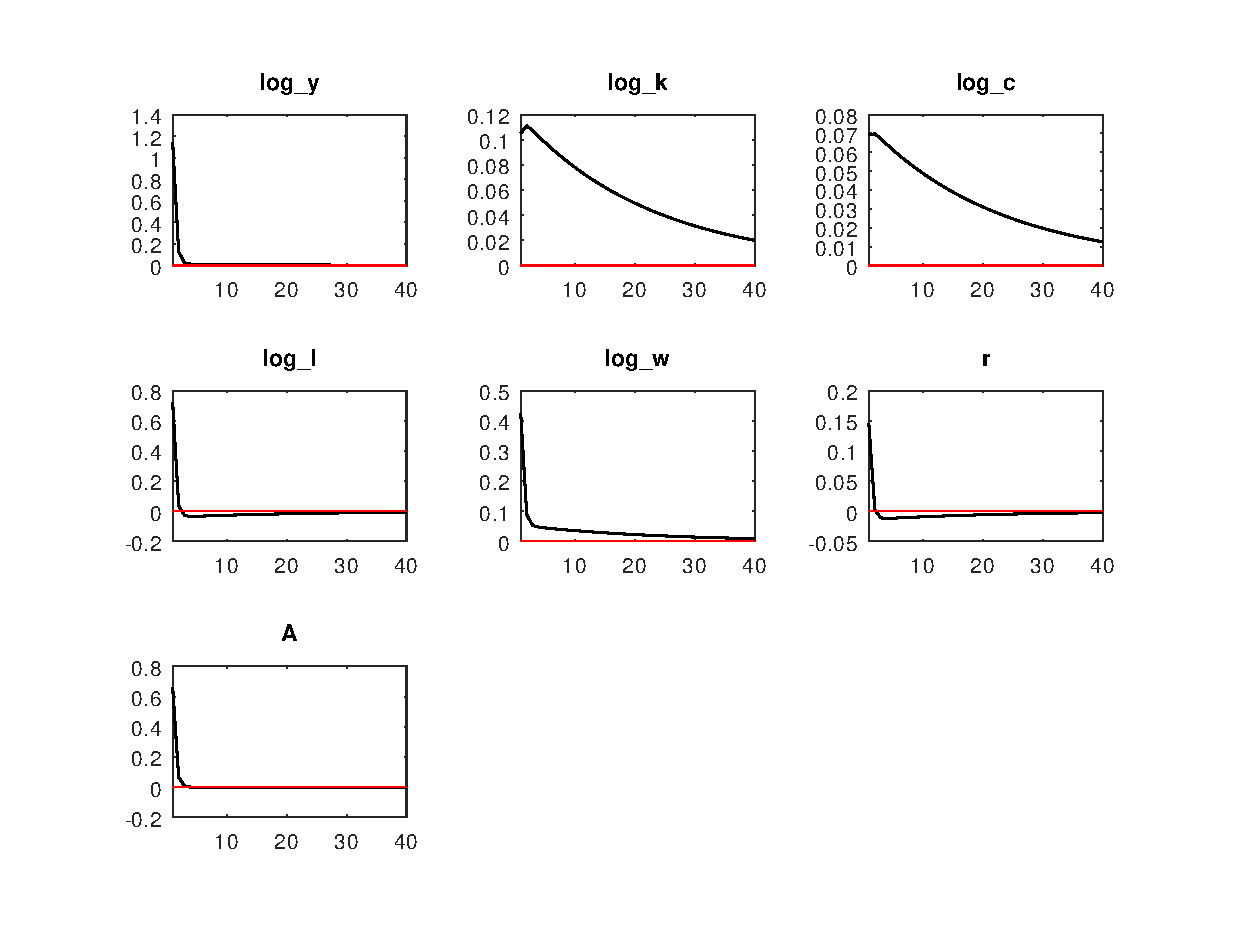
\includegraphics[width=0.80\textwidth]{RBCt_IRF_eps_A}
	
	\label{fig:rbcefectodynareptftransitorio}
\end{figure}
\renewcommand{\rgcaptioneq}{\rgcaption{Efecto de un shock de oferta transitorio en un modelo del ciclo real básico\footnote{Íbidem.}}}
\begin{center}
	\rgcaptioneq
\end{center}

\begin{figure}[!htbp]
	\psfrag{log_y}[1][][0.5][0]{${\log(y)}$}
	\psfrag{log_k}[1][][0.5][0]{${\log(k)}$}
	\psfrag{log_c}[1][][0.5][0]{${\log(c)}$}
	\psfrag{log_l}[1][][0.5][0]{${\log(l)}$}
	\psfrag{log_w}[1][][0.5][0]{${\log(w)}$}
	\psfrag{r}[1][][0.5][0]{${r}$}
	\psfrag{A}[1][][0.5][0]{${A}$}
	\centering 
	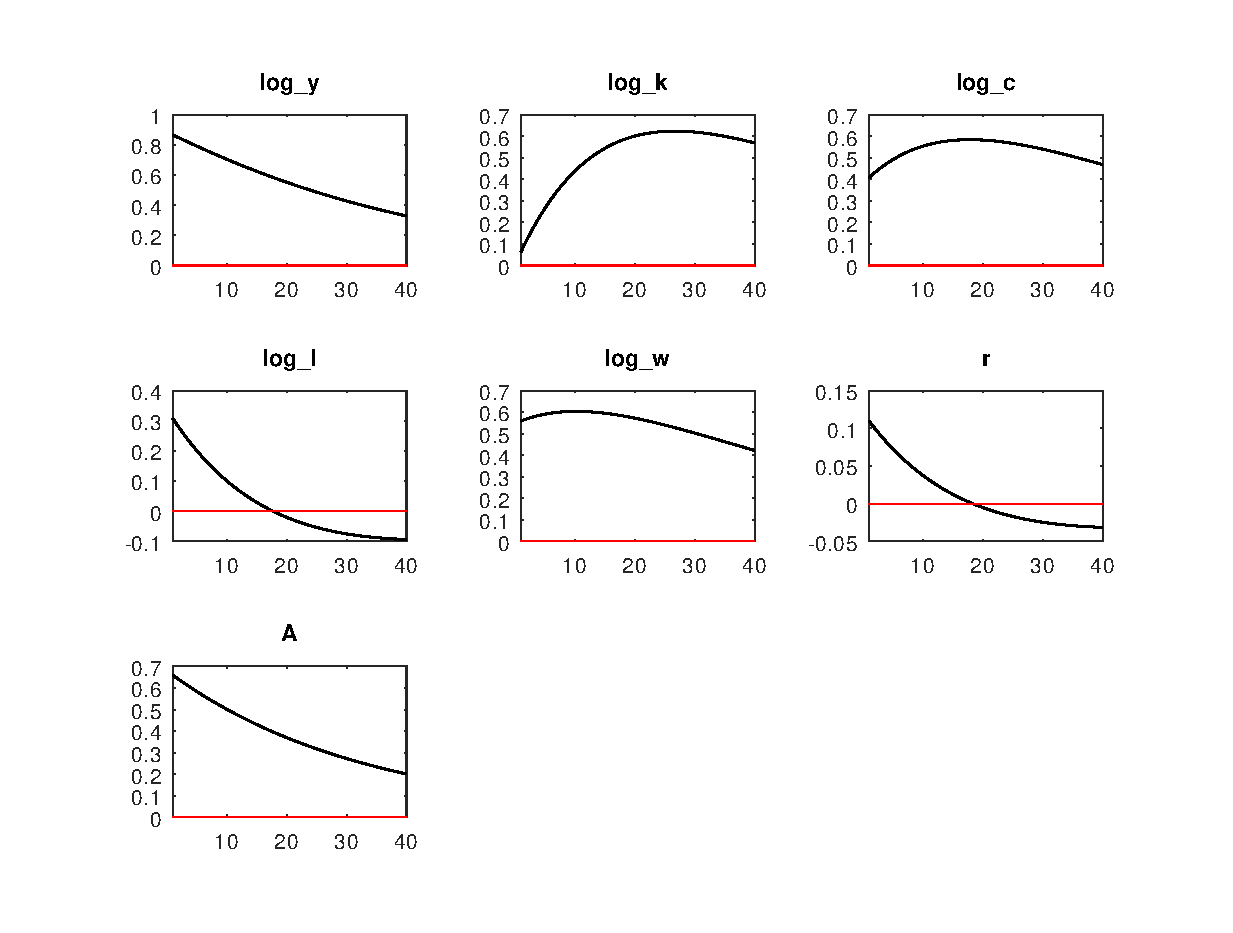
\includegraphics[width=0.80\textwidth]{RBCp_IRF_eps_A}

	\label{fig:rbcefectodynareptfpermanente}
\end{figure}
\renewcommand{\rgcaptioneq}{\rgcaption{Efecto de un shock de oferta permanente en un modelo del ciclo real básico\footnote{Estimado con modelo RBC\_Baseline.mod de \href{https://github.com/JohannesPfeifer/DSGE_mod}{Repositorio de modelos DSGE en Dynare de Johannes Pfeifer.}}.}}
\begin{center}
\rgcaptioneq
\end{center}


\begin{figure}[!htpb]
	\psfrag{log_y}[1][][0.5][0]{${\log(y)}$}
	\psfrag{log_k}[1][][0.5][0]{${\log(k)}$}
	\psfrag{log_c}[1][][0.5][0]{${\log(c)}$}
	\psfrag{log_l}[1][][0.5][0]{${\log(l)}$}
	\psfrag{log_w}[1][][0.5][0]{${\log(w)}$}
	\psfrag{r}[1][][0.5][0]{${r}$}
	\psfrag{ghat}[1][][0.5][0]{${\hat g}$}
	\centering 
	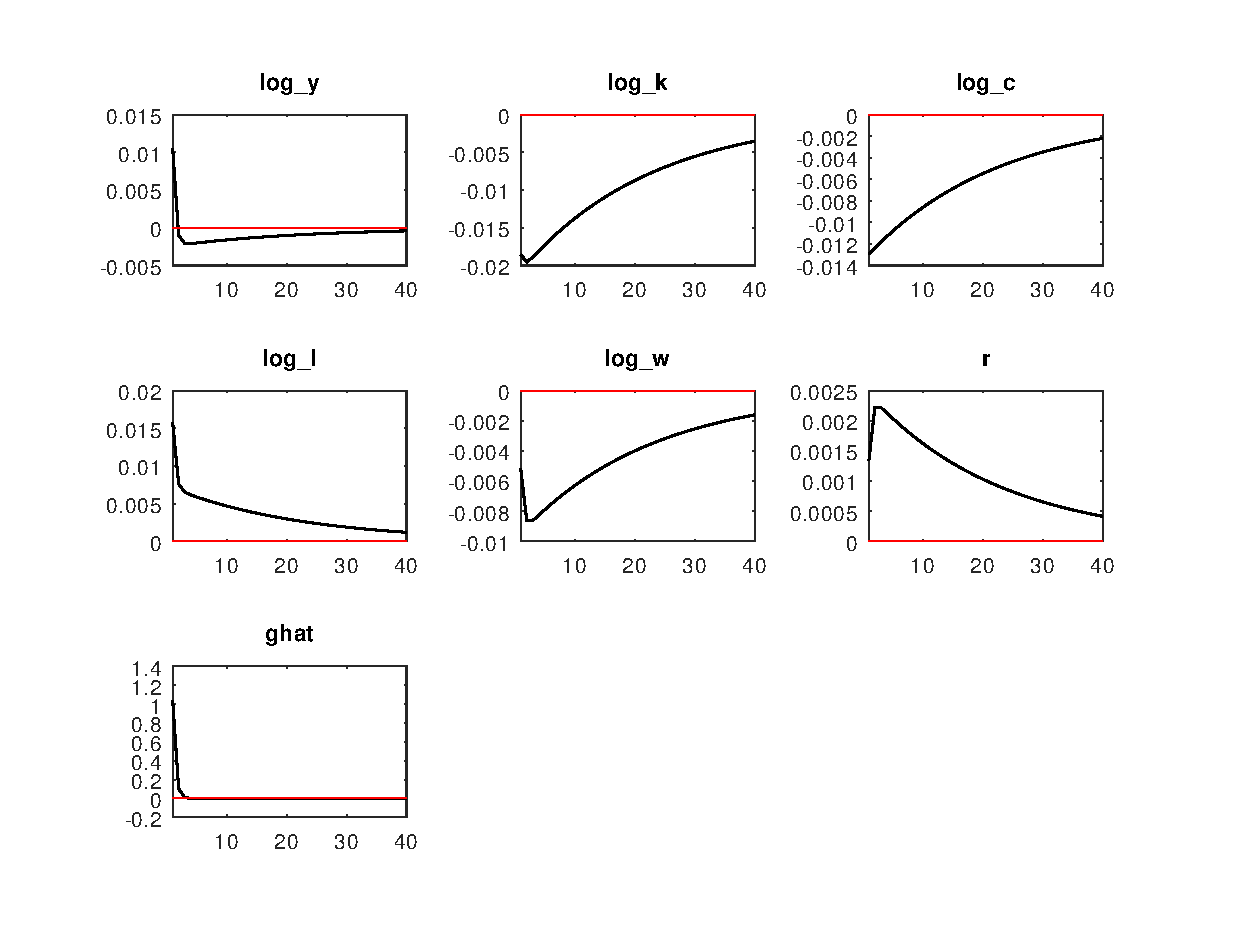
\includegraphics[width=0.80\textwidth]{RBCt_IRF_eps_g}
	\label{fig:rbcefectodynaregastotransitorio}
\end{figure}
\renewcommand{\rgcaptioneq}{\rgcaption{Efecto de un shock de gasto público transitorio en un modelo del ciclo real básico\footnote{Íbidem.}.}}
\begin{center}
	\rgcaptioneq
\end{center}


\begin{figure}[!htbp]
	\psfrag{log_y}[1][][0.5][0]{${\log(y)}$}
	\psfrag{log_k}[1][][0.5][0]{${\log(k)}$}
	\psfrag{log_c}[1][][0.5][0]{${\log(c)}$}
	\psfrag{log_l}[1][][0.5][0]{${\log(l)}$}
	\psfrag{log_w}[1][][0.5][0]{${\log(w)}$}
	\psfrag{r}[1][][0.5][0]{${r}$}
	\psfrag{A}[1][][0.5][0]{${A}$}
	\centering 
	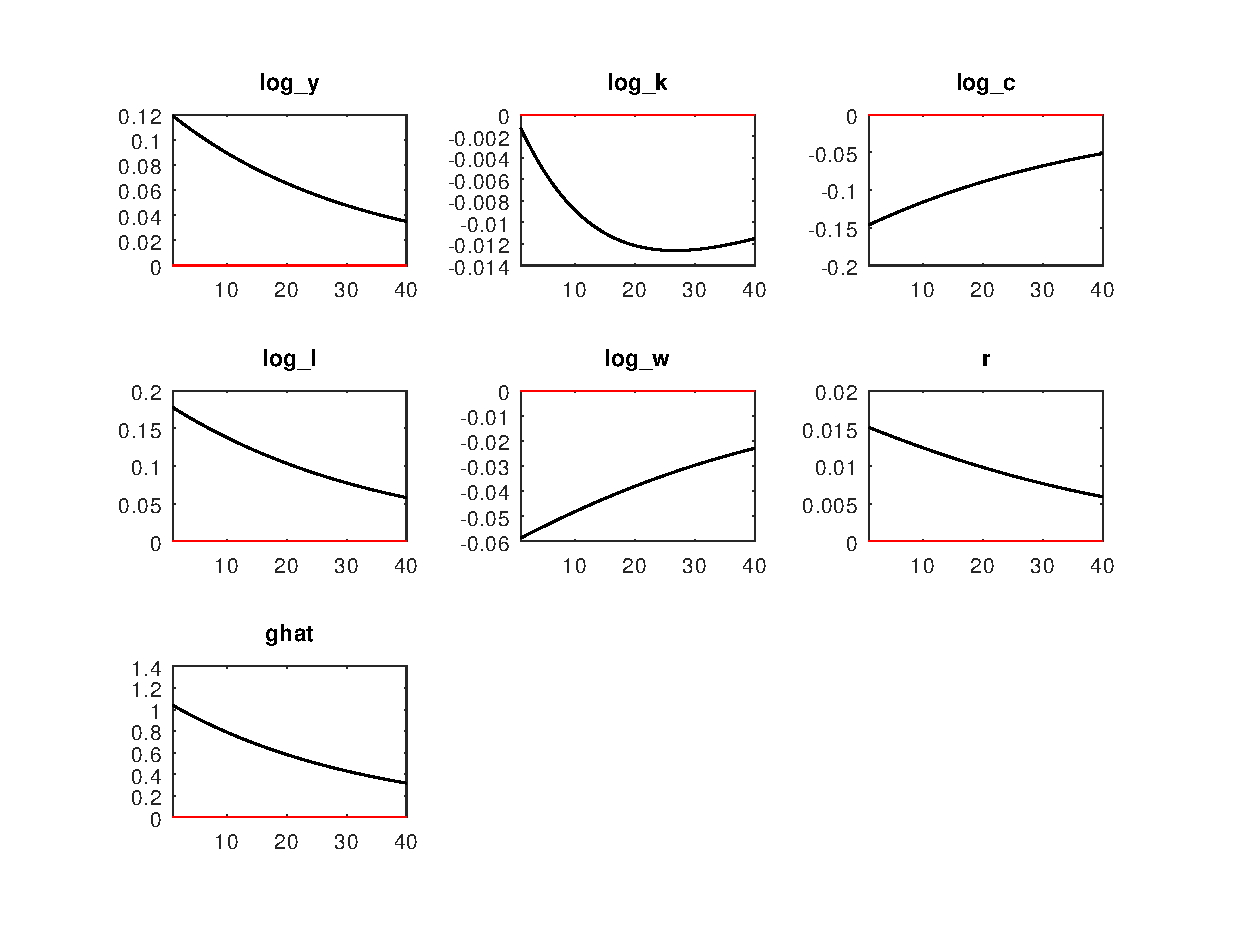
\includegraphics[width=0.80\textwidth]{RBCp_IRF_eps_g}
	
	\label{fig:rbcefectodynaregastopermanente}
\end{figure}
\renewcommand{\rgcaptioneq}{\rgcaption{Efecto de un shock de gasto público persistente en un modelo del ciclo real básico\footnote{Íbidem.}}}
\begin{center}
	\rgcaptioneq
\end{center}



\begin{tabla}{Comparación del efecto de diferentes shocks sobre el trabajo en un modelo RBC básico.}{resumenefectostrabajo}
	\begin{tabular}{l | c | c}
					   & Transitorio & Permanente \\ \hline
Shock de productividad & Aumento fuerte: $|\text{ES}+\text{ED}_i| >> \text{ER}_d$ & Aumento moderado $|\text{ES}+\text{ED}_i| > \text{ER}_d$ \\ \hline
Shock de gasto público & Aumento mínimo $|\text{ES}+\text{ED}_i| = 0 < \text{ER}_d$ & Aumento moderado $|\text{ES}+\text{ED}_i| = 0 << \text{ER}_d$ \\ \hline
	\end{tabular}
\end{tabla}
\begin{axis}{4}{Fijación de precios por un productor $i$ y posterior aumento del mark-up ante una caída de la demanda agregada y un precio que se mantiene rígido.}{$y_t(i)$}{$p_t(i)$}{ajustecantidades}
	% Curva de coste marginal
	\draw[thick] (0,0.5) to [out=0, in=220](4,2.9);
	\node[right] at (4,2.9){\tiny CMg};
	
	% Demanda inicial
	\draw[thick] (0,3.8) -- (4,1);
	\node[right] at (4,1){\tiny D};
	
	% Ingreso marginal inicial
	\draw[-] (0,3.8) -- (3.7,0);
	\node[right] at (3.7,0.2){\tiny IMg};
	
	% Cantidad de equilibrio inicial
	\draw[dashed] (2.34,0) -- (2.34,2.15); 
	
	% Precio de equilibrio inicial
	\draw[dashed] (2.34,2.15) -- (-1.2,2.15);
	
	% Coste marginal de equilibrio inicial
	% \draw[dashed] (2.35,1.4) -- (0,1.4);
	
	% Demanda final
	\draw[thick, color=red] (0,3.8) -- (4,0.5);
	\node[right, color=red] at (4,0.5){\tiny D'};
	
	% Ingreso marginal final
	\draw[-, color=red] (0,3.8) -- (3.2,0);
	
	% Cantidad final deseada
	\draw[dashed, color=red] (2.15,0) -- (2.15,2);
	\node[below] at (2.15,0){\tiny $y'_1$};
	
	% Precio final deseado
	\draw[dashed, color=red] (2.15,2) -- (0,2);
	
	% Coste marginal final deseado
	\draw[dashed, color=red] (2.15,1.25) -- (0,1.25);
	
	% Coste marginal final efectivo
	\draw[dotted, color=red] (2.0,1.14) -- (-1.2,1.14);
	
	% Cantidad final efectiva
	\draw[dotted, color=red] (2.0,2.16) -- (2.00,0);
	\node[below] at (1.92,-0.1){\tiny $y_1$};
	
	
	% Markup aplicado
	\draw[decorate,decoration={brace, mirror,amplitude=3pt},xshift=-35pt,yshift=0cm] (0,2.15) -- (0,1.16) node[black,midway,xshift=-15pt, yshift=0cm] {\tiny $\mu$ aplicado};
	
	% Markup deseado
	\draw[decorate,decoration={brace, mirror,amplitude=3pt},xshift=-5pt,yshift=0cm] (0,2) -- (0,1.25) node[black,midway,xshift=-15pt, yshift=0cm] {\tiny $\mu$ deseado};
\end{axis}

En la situación de equilibrio inicial, la empresa iguala ingreso marginal con coste para determinar la cantidad producida, y después iguala el precio con el corresponde para esa cantidad demandada. Cuando la demanda se reduce por un shock nominal o de preferencias, la curva de demanda se desplaza a la izquierda (línea roja gruesa). Dado que el precio se mantiene rígido, la empresa vende una cantidad $y_1$, que es la correspondiente a la nueva demanda para es precio. Sin embargo, la cantidad que iguala la nueva función de ingreso marginal con el coste marginal es $y_1'$, que es mayor a $y_1$. El precio que fijaría la empresa sería inferior al fijado inicialmente, y el coste marginal mayor al incurrido con la nueva demanda y precio fijo, dado que se produciría una cantidad mayor. Todo ello resulta en un mark-up aplicado mayor al que la empresa desearía aplicar para cumplir con la condición de óptimo de primer orden del problema de maximización de beneficios.






\preguntas

\seccion{Test 2015}

\textbf{21.} Considere un modelo de ciclo real y agente representativo de dos periodos $t$ y $t+1$. Suponga que en $t$ se produce un shock consistente en un desplazamiento paralelo y hacia arriba de la función de producción de carácter permanente. Indique cuál de las siguientes opciones es \textbf{falsa}:

\begin{itemize}
	\item[a] En el periodo $t$ se elevará el consumo, pero se reducirá la cantidad ofrecida de trabajo.
	\item[b] En el período $t+1$ se elevará el consumo, pero se reducirá la cantidad ofrecida de trabajo.
	\item[c] El ahorro no se alterará en ninguno de los dos periodos.
	\item[d] Se producirá un incremento del consumo presente junto con una reducción del consumo futuro debido al efecto sustitución intertemporal desencadenado por el shock de la función de producción.
\end{itemize}

\seccion{Test 2014}

\textbf{22.} Una perturbación uni-periódica al alza del gasto público, en el contexto del modelo básico del ciclo real:
\begin{itemize}
	\item[a] Es imposible porque este modelo no considera tal posibilidad.
	\item[b] Disminuirá levemente el stock de capital.
	\item[c] Desencadenará un ritmo progresivamente creciente del empleo.
	\item[d] Elevará el stock de capital a corto plazo.
\end{itemize}

\seccion{Test 2011}

\textbf{17.} Según la Teoria del Ciclo Real, una perturbación transitoria tecnológica positiva provoca:
\begin{itemize}
	\item[a] Un aumento en el nivel de producción y un aumento en el empleo, siendo el segundo superior al primero, por lo que disminuye la productividad del trabajo.
	\item[b] Un aumento en el nivel de producción y en el empleo, siendo el primero superior al segundo, por lo que aumenta la productividad del trabajo.
	\item[c] Un aumento en el consumo y una disminución en el ahorro (inversión).
	\item[d] Un aumento en la inversión, a costa de una disminución en el consumo.
\end{itemize}

\seccion{Test 2008}

\textbf{15.} Supongamos un modelo básico del ciclo real, de familias optimizadores en ocio y consumo, y de empresas optimizadores con una función de producción Cobb-Douglas. Si se produce un shock no anticipado de tal modo que mejora transitoriamente la productividad total de factores:
\begin{itemize}
	\item[a] El tipo de interés real disminuirá ligeramente para volver rápidamente a su valor de equilibrio.
	\item[b] El salario real disminuye, mostrando una cierta persistencia.
	\item[c] Los hogares disminuirán permanentemente la tasa de ahorro.
	\item[d] El empleo aumenta, pero sólo transitoriamente.
\end{itemize}

\seccion{Test 2007}

\textbf{18.} Si los precios son completamente flexibles, el nivel de producción fluctúa debido a la existencia de choques de productividad y el Banco Central mantiene constante la oferta de dinero, entonces si el nivel de producción aumenta, el nivel de precios:

\begin{itemize}
	\item[a] Permanecerá constante.
	\item[b] Subirá porque la demanda de dinero sube cuando el nivel de producción aumenta.
	\item[c] Caerá porque la demanda de dinero sube cuando el nivel de producción aumenta.
	\item[d] Fluctuará, pero no de forma no relacionada con las fluctuaciones de la producción.
\end{itemize}

\seccion{Test 2004}

\textbf{20.} En el contexto de la teoría de los ciclos económicos, y respecto a la evidencia empírica disponible, entre las siguientes afirmaciones:

\begin{itemize}
	\item[i)] Las fluctuaciones asociadas al ciclo económico las predice la teoría neoclásica del crecimiento si los shocks a la productividad total de los factores son persistentes y de magnitud adecuada.
	\item[ii)] Dos tercios de las fluctuaciones en el producto agregado son atribuibles, en el marco de la teoría neoclásica del crecimiento, a variaciones en el factor trabajo.
	\item[iii)] El consumo de bienes no duraderos es fuertemente procíclico y fluctúa tanto como el producto agregado en términos porcentuales.
	\item[iv)] Las fluctuaciones asociadas al ciclo económico no pueden ser un fenómeno de equilibrio y por tanto, la teoría del equilibrio general no es útil para su estudio.
\end{itemize}

\begin{itemize}
	\item[a] Solamente la ii) y la iii) son verdaderas.
	\item[b] Solamente la iii) y la iv) son verdaderas.
	\item[c] Solamente la i) y la ii) son verdaderas.
	\item[d] Solamente la ii) y la iv) son verdaderas.
\end{itemize}

\notas

\textbf{2015:} \textbf{21.} D

\textbf{2014:} \textbf{22.} B

\textbf{2011:} \textbf{17.} B

\textbf{2008:} \textbf{15.} D

\textbf{2007:} \textbf{18.} C

\textbf{2004:} \textbf{20.} C


Importante contar hechos estilizados de las fluctuaciones.

\bibliografia

Mirar en Palgrave:
\begin{itemize}
	\item business cycles
	\item business cycle measurement
	\item international real business cycles
	\item monetary business cycles models (sticky prices and wages)
	\item monetary business cycles (imperfect information)
	\item monetary transmission mechanism
    \item natural rate and market rate of interest
    \item real business cycles
    \item real rigidities
    \item sticky wages and staggered wage setting
    \item stylized facts
    \item welfare costs of business cycles
\end{itemize}

Álvarez, L.; Gómez-Loscos, G. \textit{A Menu on Output Gap Estimation} (2017) Banco de España. Documentos de Trabajo -- En carpeta del tema

Ball, Mankiw (2002) \textit{The NAIRU in theory and practice.} Journal of Economic Perspectives

Basu, S.: Taylor, A. M. \textit{Business Cycles in International Historical Perspective} (1999) Journal of Economic Perspectives -- En carpeta del tema

Blanchard, O.; Gali, J. \textit{Real Wage Rigidites and the New Keynesian Model} (2007) Journal of Money, Credit and Banking -- En carpeta del tema

Christiano, L. J; Eichenbaum, M. S.; Evans, C. L. \textit{Monetary Policy Shocks: What Have We Learned and to What End?} (1999) Handbook of Macroeconomics. Vol. 1 -- En carpeta del tema

Christiano, L. J; Eichenbaum, M. S.; Evans, C. L. \textit{Nominal Rigidities and the Dynamic Effects of a Shock to Monetary Policy} (2005) Journal of Political Economy -- En carpeta del tema 

Christiano, L. J.; Eichenbaum, M. S.; Trabandt, M. \textit{On DSGE Models} (2018) Journal of Economic Perspectives: Summer 2018 -- En carpeta del tema

Fabozzi, F. J. \textit{Handbook of Fixed Income Securities} Ch. 5(Macro-Economic dynamics and the corporate bond market)

Gomes, S.; Jacquinot, P.; Pisani, M. (2010) \textit{The EAGLE. A model for policy analysis of macroeconomic interdependence in the Euro Area} ECB Working Paper-- En carpeta del tema

Groth, C. \textit{Chapter 29. The real business cycle theory} Lecture notes. \url{http://www.econ.ku.dk/okocg/VM/VM11/Lectures\%20and\%20lecture\%20notes/Ch29-2011-1.pdf} -- En carpeta del tema

Groth, C. \textit{Chapter 29. Business fluctuations} Lecture notes. \url{http://www.econ.ku.dk/okocg/VM/VM-general/Kapitler\%20til\%20bog/Ch29-2016-1.pdf} -- En carpeta del tema


Heertje, A.; Heemeijer, P. (2002) \textit{On the Origin of Samuelson's Multiplier-Accelerator Model} Duke University Press -- En carpeta del tema

Heijdra, B. J. \textit{Foundations of Modern Macroeconomics} (2017) 3rd ed. -- En carpeta Macro

Journal of Economic Perspectives. \textit{Vol. 13 N. 2} (1999) Spring

King, R. G.; Rebelo, S. T. \textit{Resuscitating Business Cycles} (1999) Handbook of Macroeconomics -- En carpeta del tema

Kydland, F. E.; Prescott, E. C. \textit{Business Cycles: Real Facts and a Monetary Myth}

Kydland, F. E. \textit{Quantitative Aggregate Theory} (2004) Nobel Prize Lecture -- En carpeta del tema

Lucas, R. \textit{An Equilibrium Model of the Business Cycle} (1975) Journal of Political Economy -- En carpeta del tema

Mankiw, G. \textit{Real Business Cycles: A New Keynesian Perspective} (1989) Journal of Economic Perspectives -- En carpeta del tema

Pfeifer, J. \textit{DSGE\_Mod: A collection of Dynare Models} \url{https://github.com/JohannesPfeifer/DSGE_mod}

Prescott, E. C. \textit{Theory Ahead of Business Cycle Measurement} (1986) Federal Reserve Bank of Minneapolis - Quarterly Review (Fall 1986) -- En carpeta del tema

Prescott, E. C. \textit{The Transformation of Economic Policy and Research} (2004) Nobel Prize Lecture -- En carpeta del tema

Romer, D. \textit{Advanced Macroeconomics} 4a, 3a, 2a eds. -- En carpeta Macro

Serletis, Apostolos, and David Krause. \textit{Nominal Stylized Facts of Business Cycles.} In Federal Reserve Bank of St. Louis Review. 1996.

Smets, F.; Wouters, R. \textit{An Estimated Stochastic Dynamic General Equilibrium Model of the Euro Area} (2002) ECB Working Paper Series -- En carpeta del tema

Sims, E. (2015) \textit{Graduate Macro Theory II: Fiscal Policy in the RBC Model} \url{https://www3.nd.edu/~esims1/fiscal_policy_sp2015.pdf} -- En carpeta del tema

Sims, E. \textit{Graduate Macro Theory II: The Real Business Cycle Model} (2016) -- En carpeta del tema

\end{document}
